\chapter{Results analysis}
\label{chapter:results-analysis}

In this chapter we analyse the results produced by the four models developed in this thesis. We are going to compare its results for each of the three problems considered: free Elastica, constrained Elastica and image segmentation.~\cref{tab:models-summary} summarizes the models properties.

In the image segmentation section, we compare our results with the linear model for curvature regularization of Schoenemann.

\begin{table}[H]
\centering
\begin{tabular}{r|ccccc}
Model & Implementation & Running time & Free Ela. & Constrained Ela. & Image Seg.\\
\hline
LocalSearch (LS) & medium & slow & yes(opt) & yes & no \\
FlipFlow (FF) & hard & acceptable & yes & no & yes \\
BalanceFlow (BF) & medium & acceptable & yes & no & yes \\
GraphFlow (GF) & easy & fast & yes(opt) & yes & yes
\end{tabular}
\caption{Models summary. The qualitative attributes are relative, e.g., the GraphFlow presents the lowest running time while LocalSearch presents the highest.}
\label{tab:models-summary}
\end{table}

\section{Free Elastica}

The free Elastica problem consists in to find a shape with the lowest digital Elastica. The approach to solve this problem as well the two others that follow, is to iteractively evolve a initial shape to another with lower digital Elastica value. We have ran two experiments, summarized in~\cref{tab:free-elastica-parameters-summary}, to illustrate the evolution process behaviour for each of the models described in this thesis. 

The parameter $eRadius$ corresponds to the radius of the disk used to compute the balance coefficient in the FlipFlow,BalanceFlow and GraphFlow models. The $vRadius$ corresponds to the radius parameter of the II curvature estimator to compute the digital Elastica in the plots of~\cref{fig:plots-free-elastica-general} and in the validation function of GraphFlow and LocalSearch.

\begin{table}
\centering
\begin{tabular}{|c|c|c|c|c|c|c|c|c|c|}
\cline{7-10}
\multicolumn{6}{c|}{} & $LS$ & $FF,BF$ & \multicolumn{2}{|c|}{$GF$}\\
\hline
Experiment & $maxIt$ & $vRadius$ & $eRadius$ & $\alpha$ & $\beta$  & $nc$ & $m$ & $a$ & $ob$ \\
\hline
General & $400$ & $5$ & $7$ & $0.01$ & $1$  & $4$ & $5$ & $2$ & $3$ \\
\hline
\multirow{2}{*}{Radius-choice} & \multirow{2}{*}{$400$} & \multirow{2}{*}{$5$} & $7$ & \multirow{2}{*}{$0.001$} & \multirow{2}{*}{$1$}  & \multirow{2}{*}{4} & $5$ & \multirow{2}{*}{$2$} & \multirow{2}{*}{$3$} \\
& &  & $12$ &  & & & $10$ & &  \\
\hline
\end{tabular}
\caption{Parameters listing for the constrained Elastica experiments. The headers $LS,FF,BF,GF$ highlights parameters that are exclusive for the LocalSearch, FlipFlow, BalanceFlow and GraphFlow models, respectively.}
\label{tab:free-elastica-parameters-summary}
\end{table}

\subsection{General experiment}

  The General experiment executes each model using the listed parameters in~\cref{tab:free-elastica-parameters-summary} for $5$ different parametric shapes. The results for the General experiment is shown in~\cref{fig:results-free-elastica-general}. One can check in the plots of~\cref{fig:plots-free-elastica-general} how the digital Elastica value evolves at each iteration. For this experiment we also provide~\cref{tab:rtime-free-elastica-general} with the model's respective running times.
  

We observe that both LocalSearch and GraphFlow evolves the initial shape to another closer to the optimal one, i.e., for $\alpha=0.01$, the disk of radius $10$. However, the GraphFlow model is simpler to implement and much faster than LocalSearch, as~\cref{tab:rtime-free-elastica-general} evidentiates. Even with a smaller neighborhood, the GraphFlow achieves its convergence first than LocalSearch in two ocassions, one in the square and the other in the flower evolution.

At the first iterations, FlipFlow and BalanceFlow produce shapes with lower digital Elastica energy. However, the models do not stop to evolve even if a shape of smaller perimeter and lower digital Elastica ceases to exist, and starting from this point, the digital Elastica value increases.


\begin{figure}
\center
\captionsetup{type=table}
\begin{tabular}{|l|c|c|c|c|c|}
\hline
& Pixels & LocalSearch & FlipFlow & BalanceFlow & GraphFlow \\
\hline
Triangle & 8315 & 1.7s/it & 0.4s/it & 0.38s/it & 0.14s/it\\
Square & 12769 & 1s/it & 0.51s/it & 0.47s/it & 0.12s/it\\
Ellipse  & 10038 & 1.3s/it & 0.64s/it & 0.57s/it & 0.1s/it \\
Flower & 26321 & 4.7s/it & 1.23s/it & 0.94s/it & 0.14s/it\\
Bean  & 25130 & 3s/it & 1.2s/it & 1.17s/it & 0.16s/it\\
\hline
\end{tabular}
\caption{Running time and input size of the General experiment for the free Elastica.}
\label{tab:rtime-free-elastica-general} 
\end{figure}


\begin{figure}
\begin{tabular}{cccc}
LocalSearch & FlipFlow & BalanceFlow & GraphFlow\\[1em]
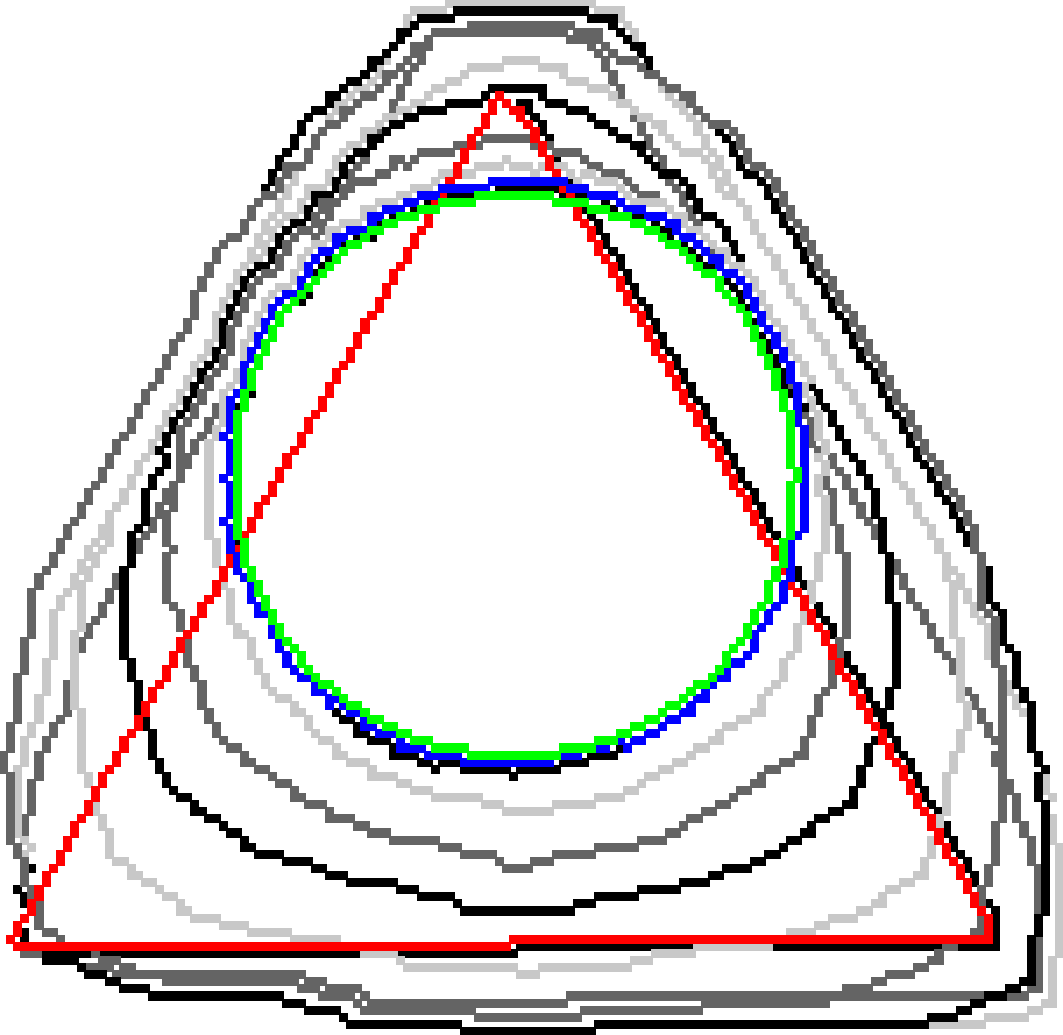
\includegraphics[scale=0.15]{figures/chapter9/free-elastica/localsearch/triangle/len_pen-0.01/radius-7/summary.pdf} & 
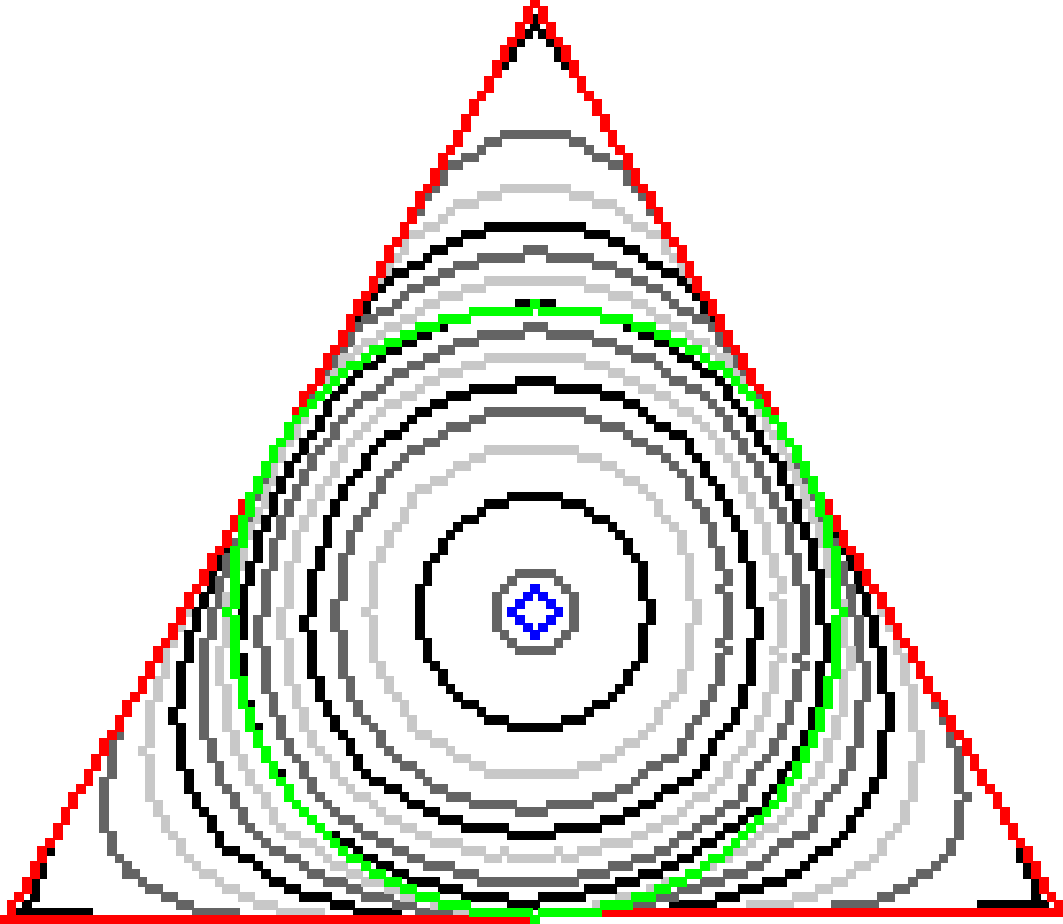
\includegraphics[scale=0.15]{figures/chapter9/free-elastica/flipflow/triangle/len_pen-0.01/radius-7/summary.pdf} &
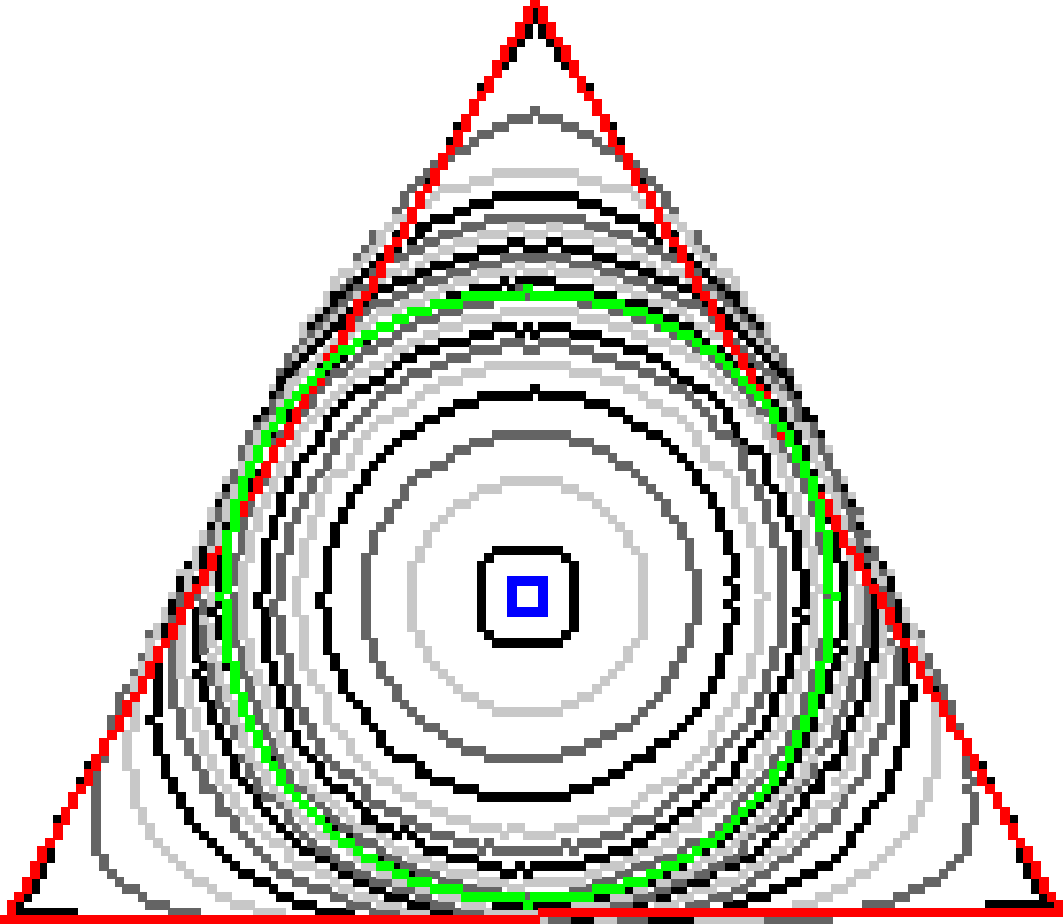
\includegraphics[scale=0.15]{figures/chapter9/free-elastica/balanceflow/triangle/len_pen-0.01/radius-7/summary.pdf} &
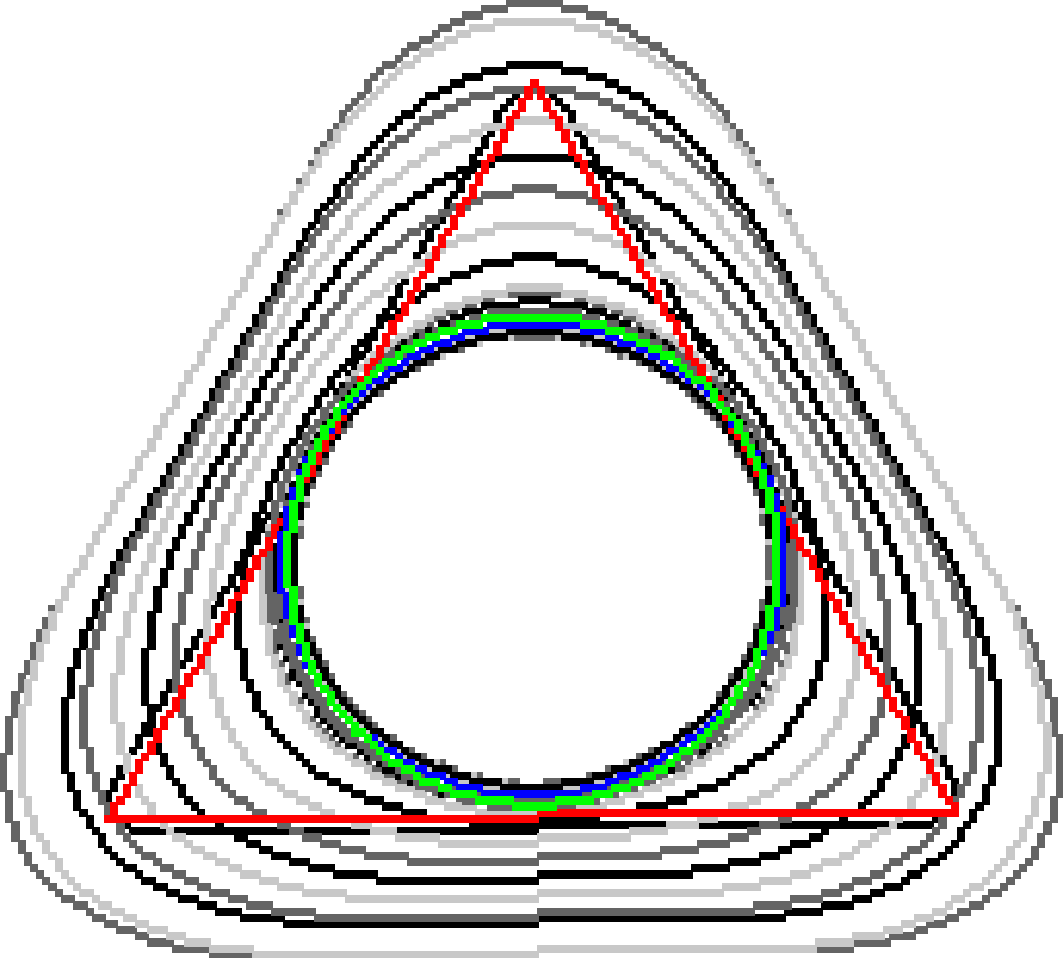
\includegraphics[scale=0.15]{figures/chapter9/free-elastica/graphflow/triangle/len_pen-0.01/radius-7/summary.pdf} \\[1em]
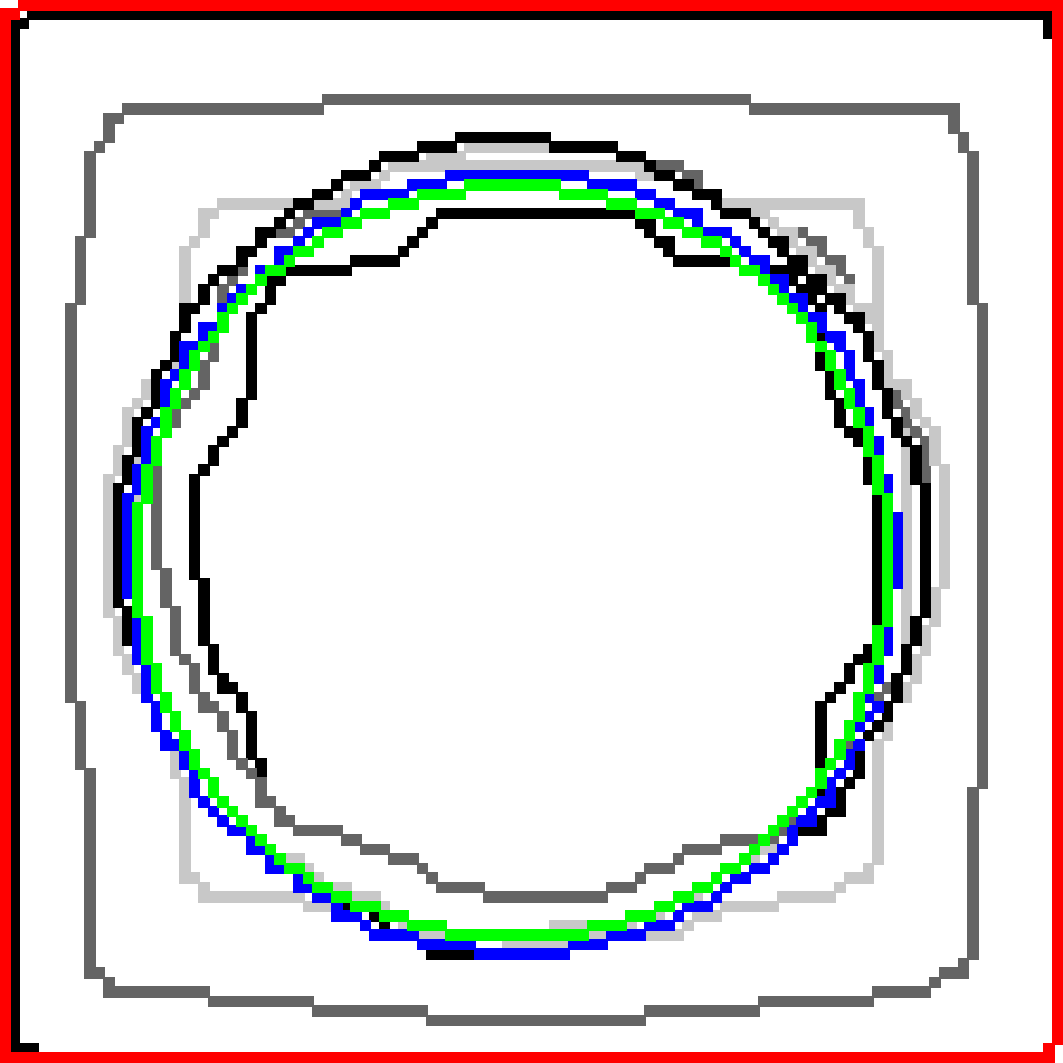
\includegraphics[scale=0.15]{figures/chapter9/free-elastica/localsearch/square/len_pen-0.01/radius-7/summary.pdf} & 
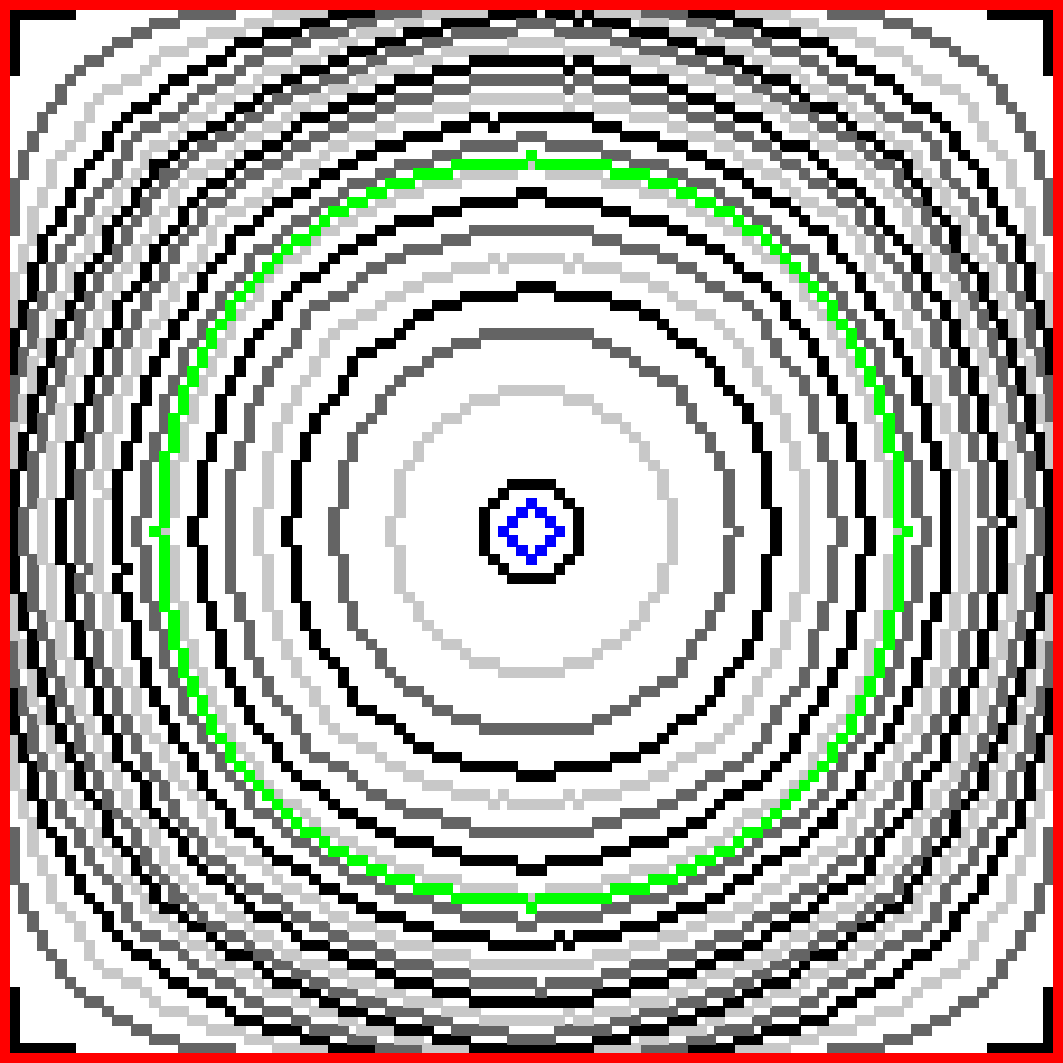
\includegraphics[scale=0.15]{figures/chapter9/free-elastica/flipflow/square/len_pen-0.01/radius-7/summary.pdf} &
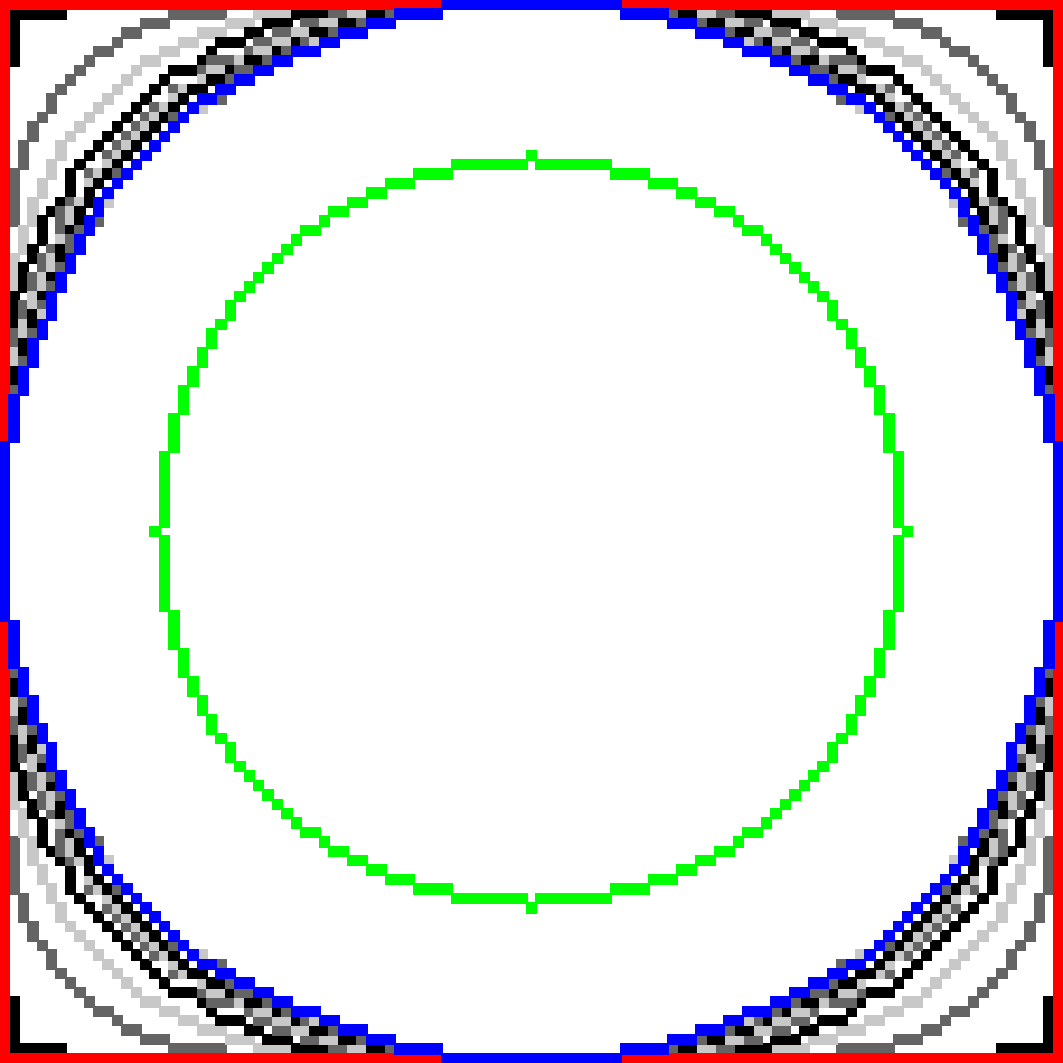
\includegraphics[scale=0.15]{figures/chapter9/free-elastica/balanceflow/square/len_pen-0.01/radius-7/summary.pdf} &
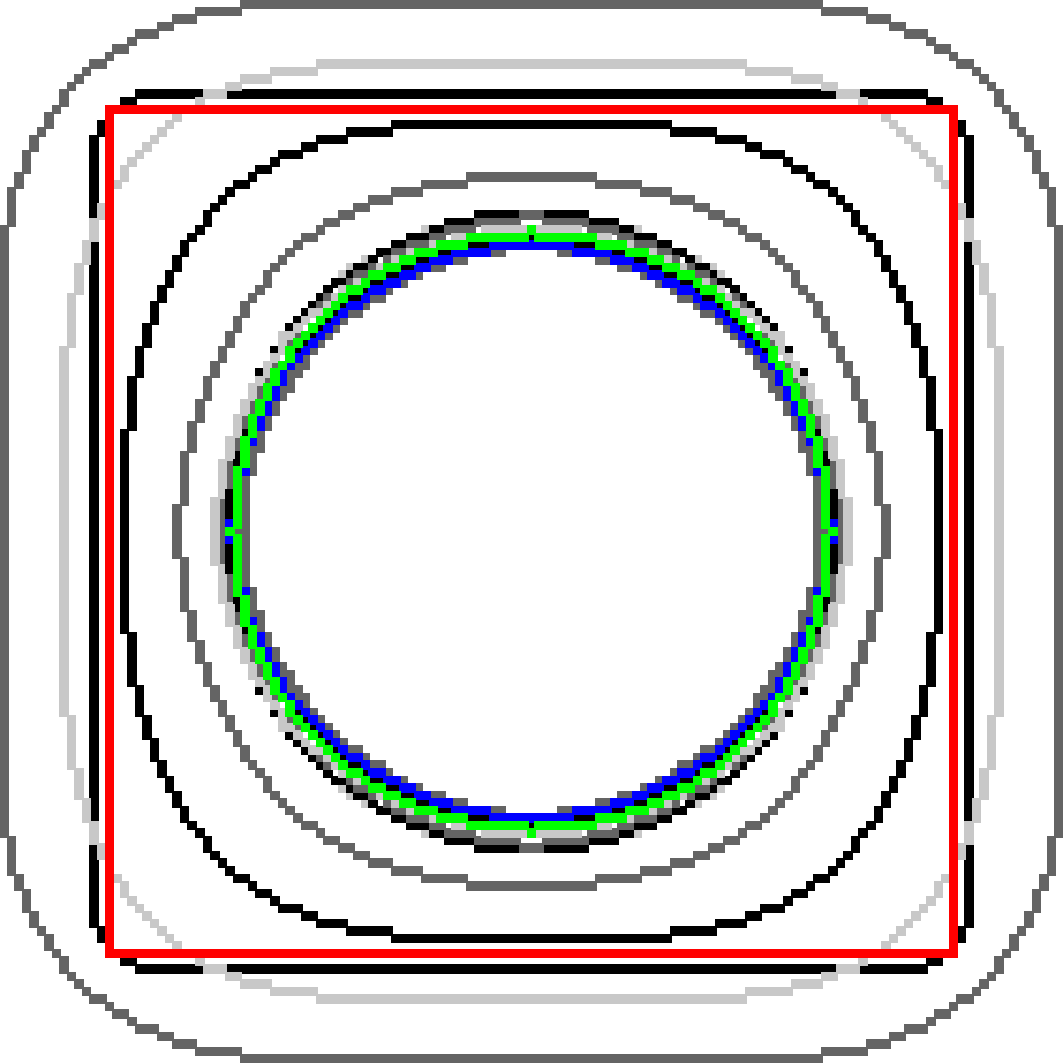
\includegraphics[scale=0.15]{figures/chapter9/free-elastica/graphflow/square/len_pen-0.01/radius-7/summary.pdf} \\[1em]
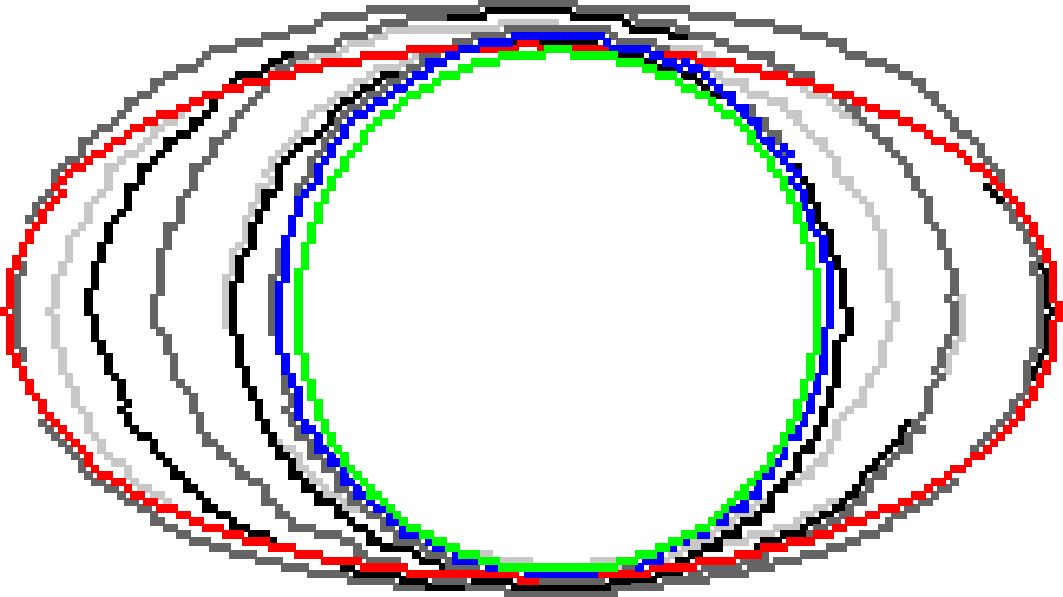
\includegraphics[scale=0.2]{figures/chapter9/free-elastica/localsearch/ellipse/len_pen-0.01/radius-7/summary.pdf} & 
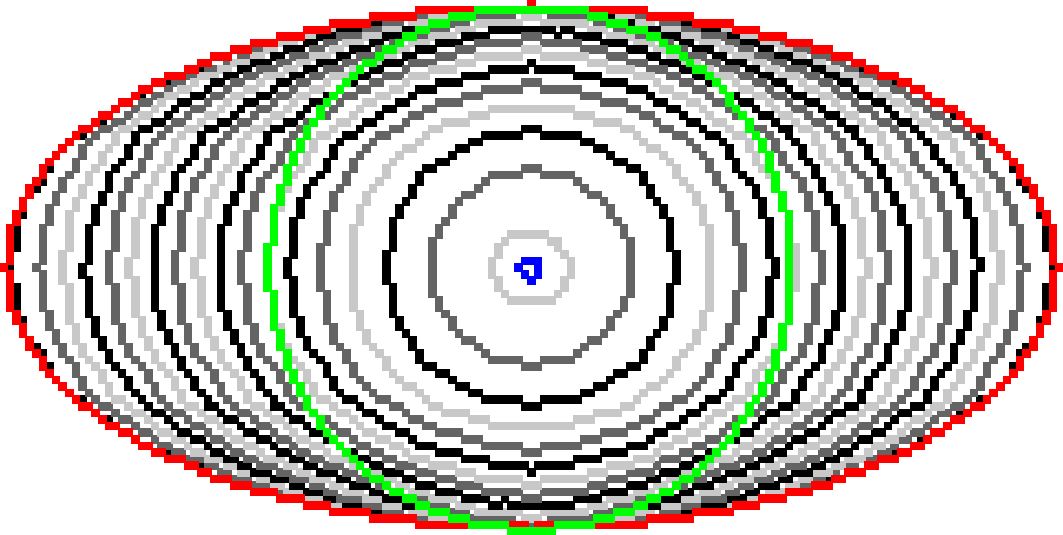
\includegraphics[scale=0.2]{figures/chapter9/free-elastica/flipflow/ellipse/len_pen-0.01/radius-7/summary.pdf} &
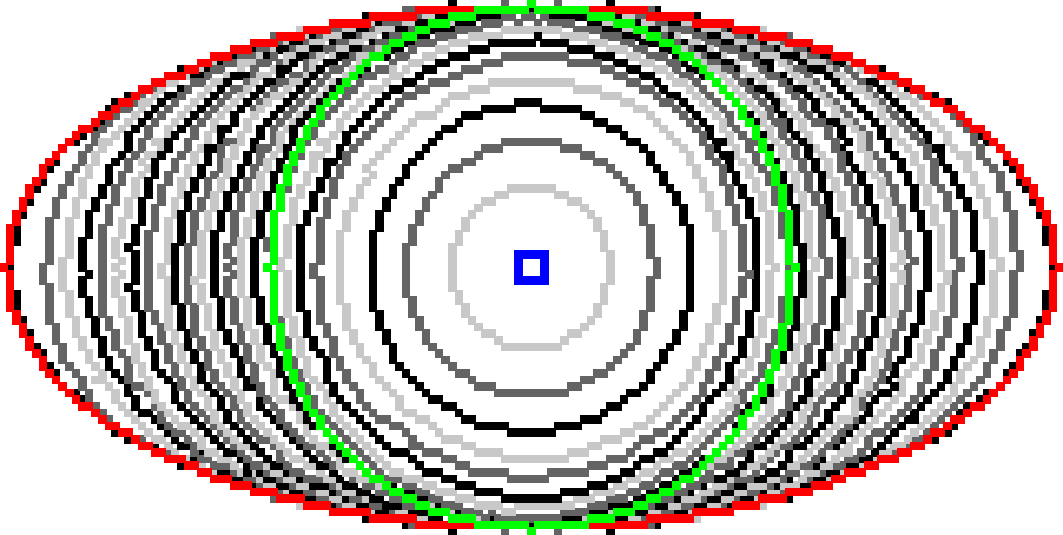
\includegraphics[scale=0.2]{figures/chapter9/free-elastica/balanceflow/ellipse/len_pen-0.01/radius-7/summary.pdf} &
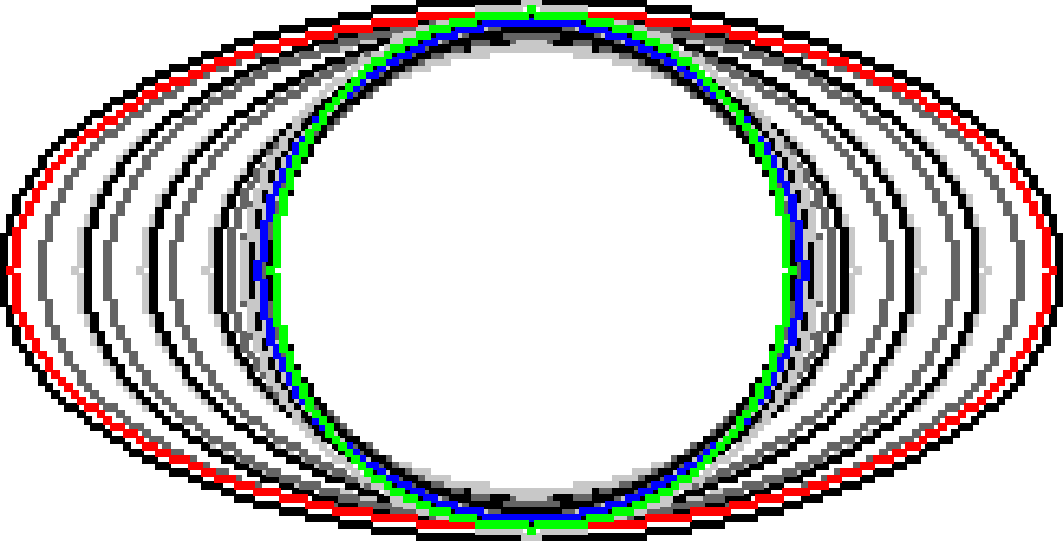
\includegraphics[scale=0.2]{figures/chapter9/free-elastica/graphflow/ellipse/len_pen-0.01/radius-7/summary.pdf} \\[1em]
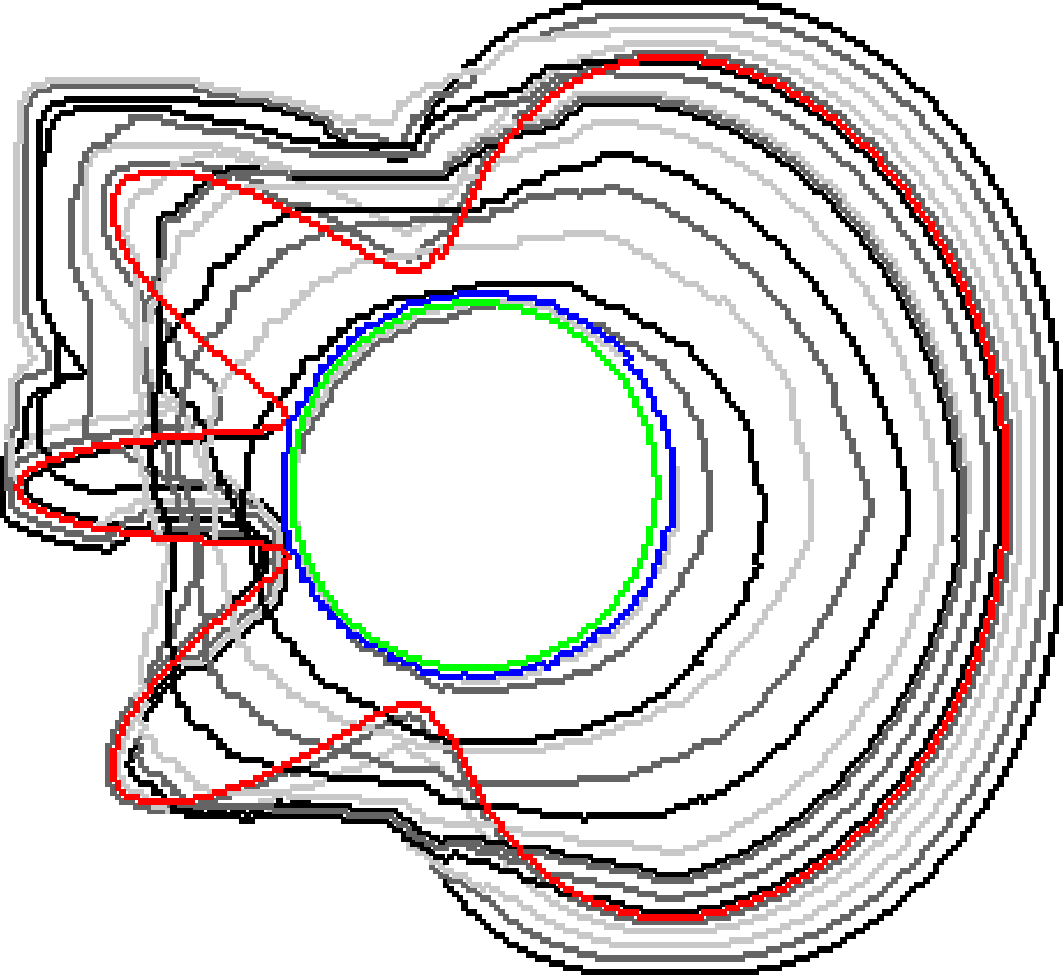
\includegraphics[scale=0.2]{figures/chapter9/free-elastica/localsearch/flower/len_pen-0.01/radius-7/summary.pdf} & 
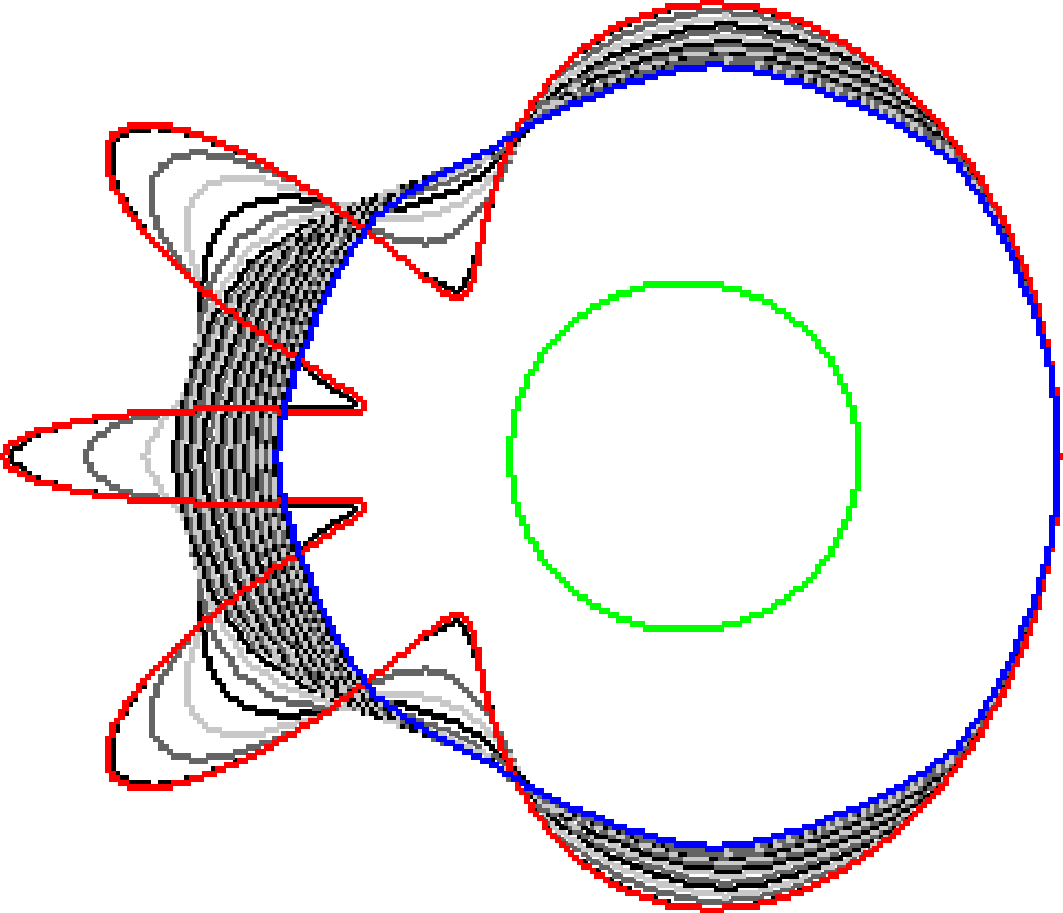
\includegraphics[scale=0.2]{figures/chapter9/free-elastica/flipflow/flower/len_pen-0.01/radius-7/summary.pdf} &
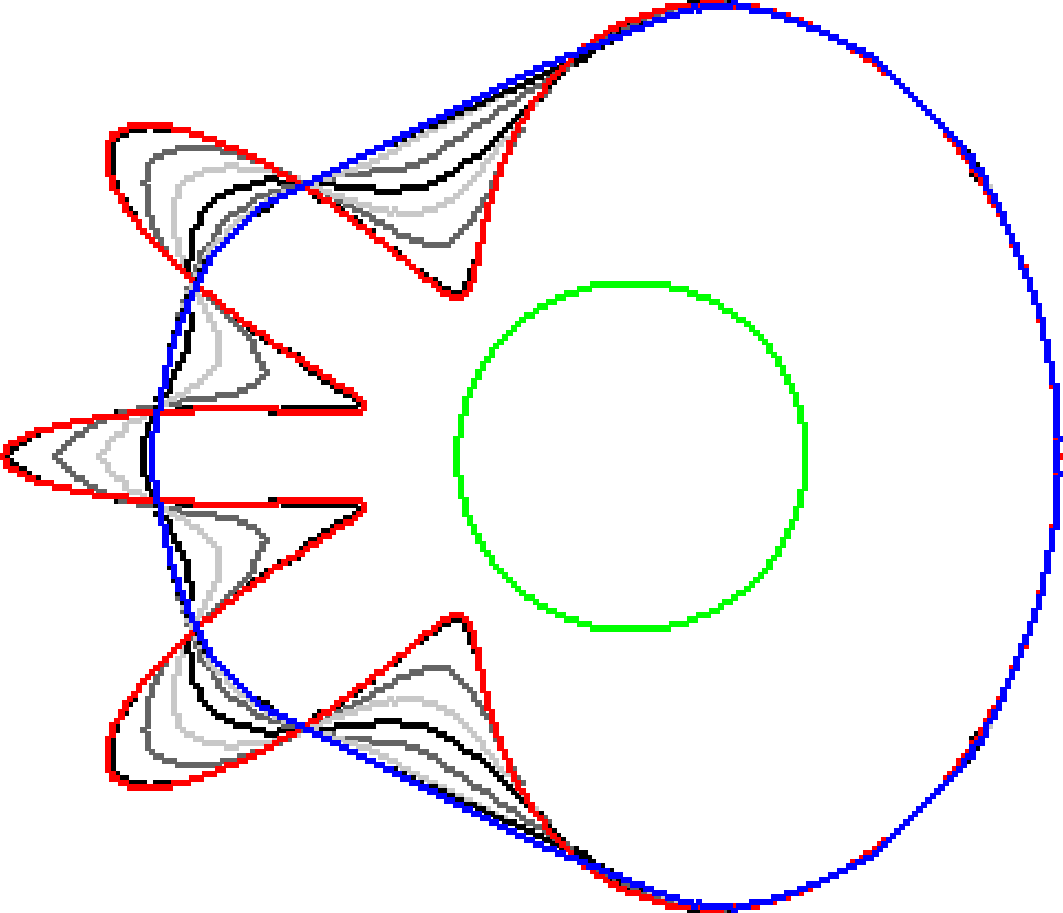
\includegraphics[scale=0.2]{figures/chapter9/free-elastica/balanceflow/flower/len_pen-0.01/radius-7/summary.pdf} &
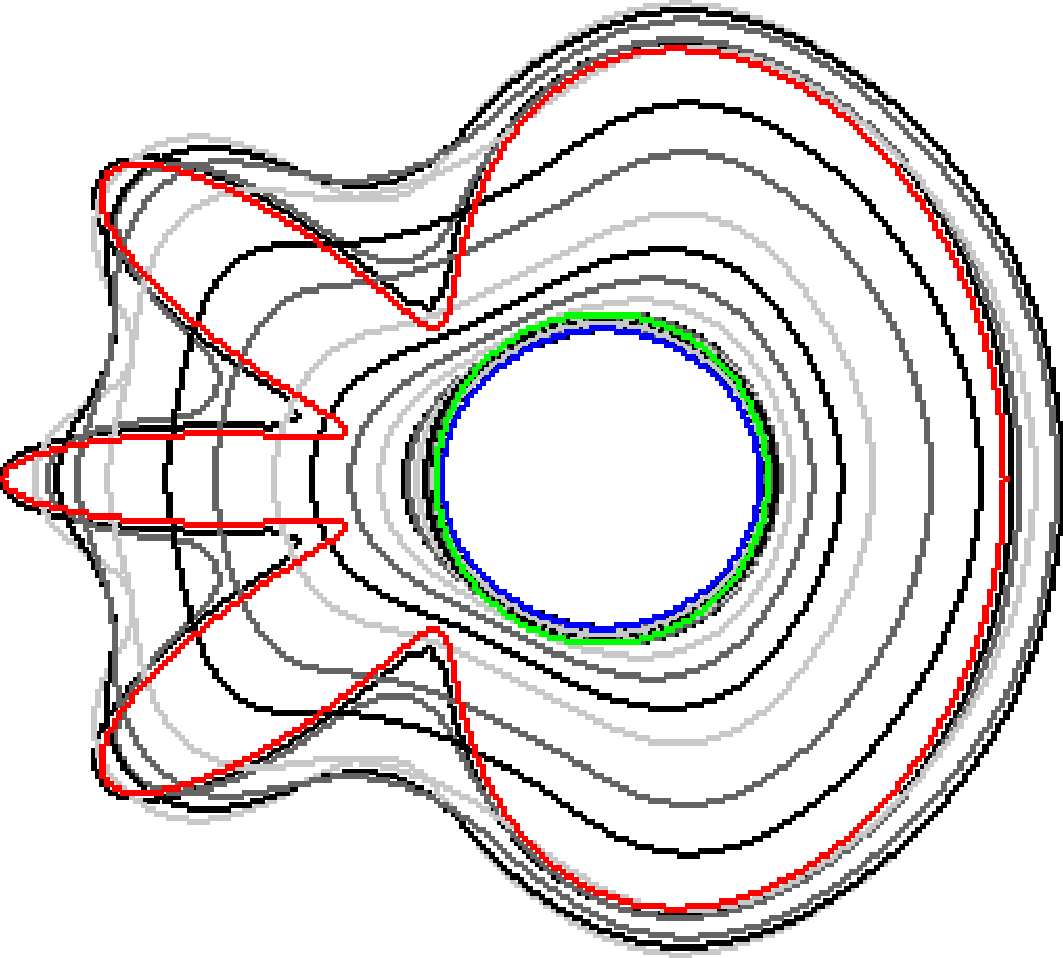
\includegraphics[scale=0.2]{figures/chapter9/free-elastica/graphflow/flower/len_pen-0.01/radius-7/summary.pdf} \\[1em]
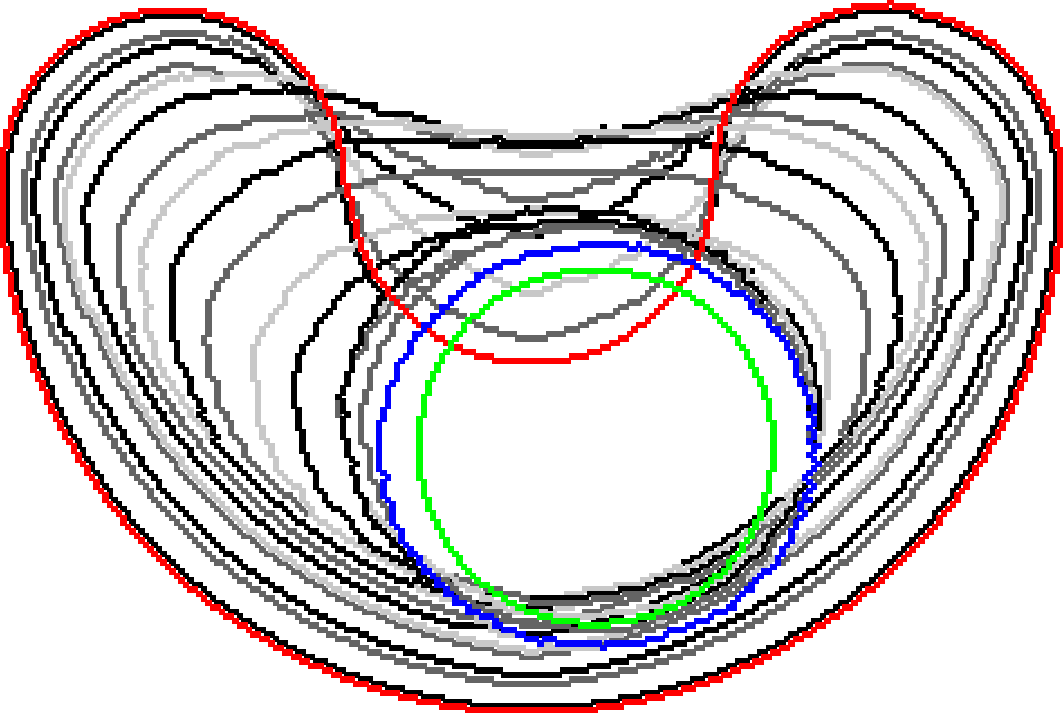
\includegraphics[scale=0.2]{figures/chapter9/free-elastica/localsearch/bean/len_pen-0.01/radius-7/summary.pdf} & 
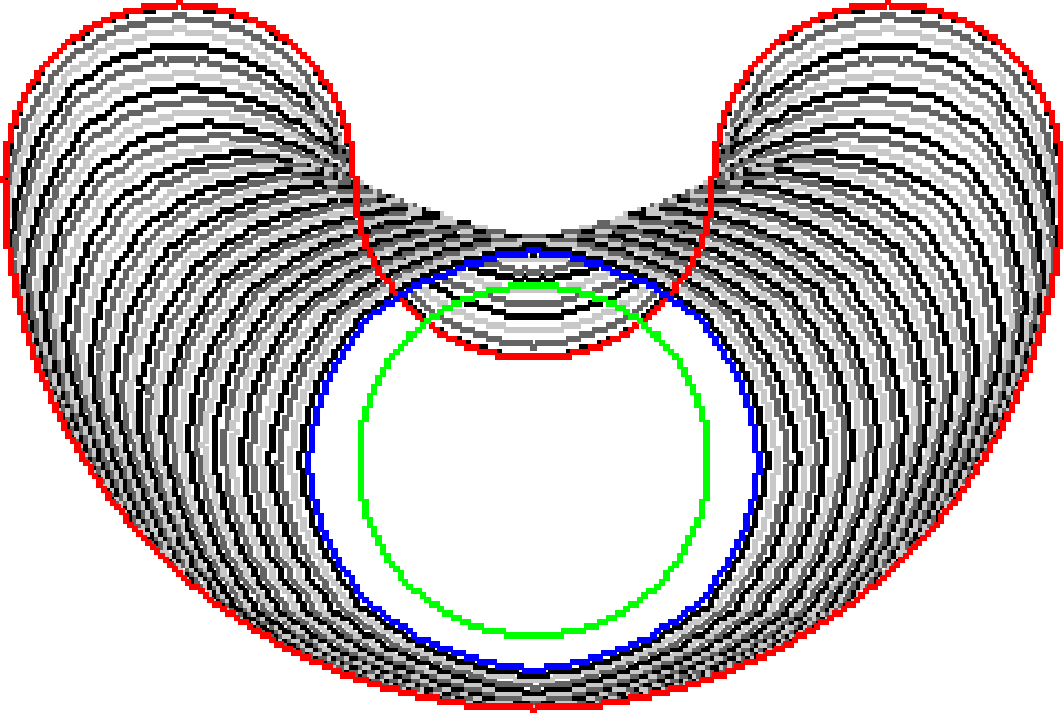
\includegraphics[scale=0.2]{figures/chapter9/free-elastica/flipflow/bean/len_pen-0.01/radius-7/summary.pdf} &
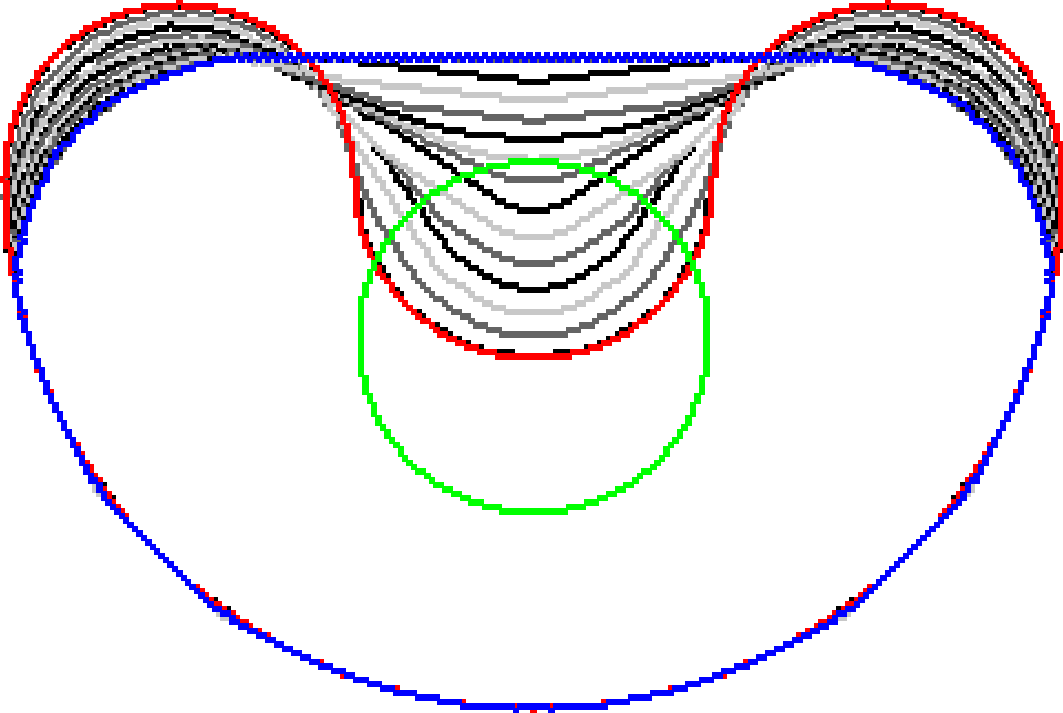
\includegraphics[scale=0.2]{figures/chapter9/free-elastica/balanceflow/bean/len_pen-0.01/radius-7/summary.pdf} &
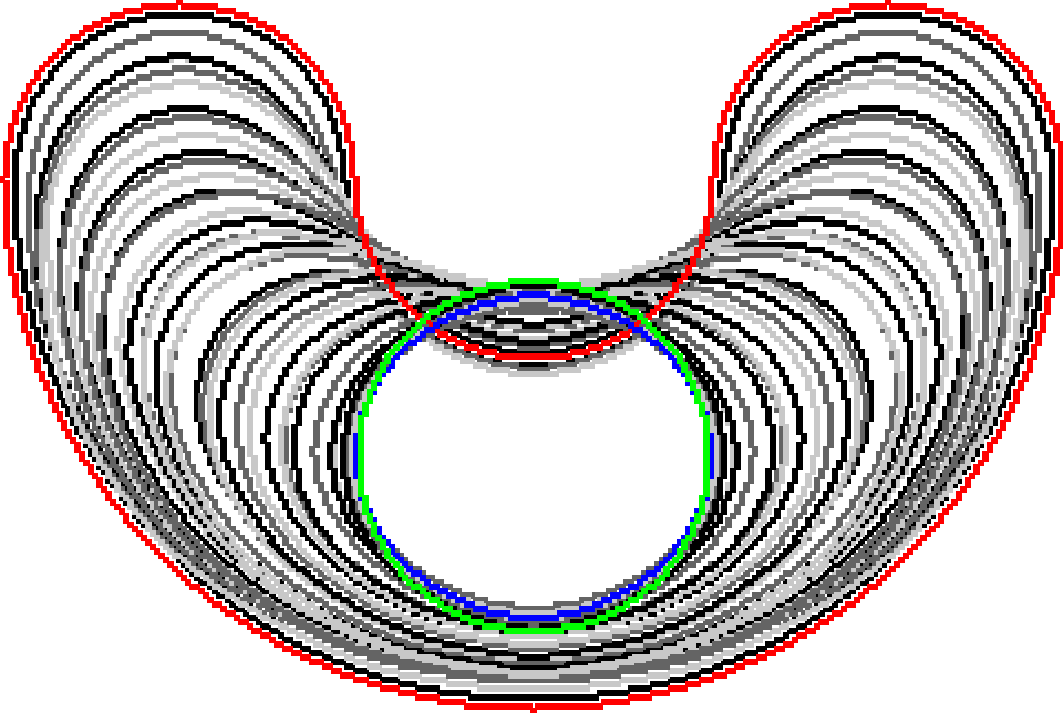
\includegraphics[scale=0.2]{figures/chapter9/free-elastica/graphflow/bean/len_pen-0.01/radius-7/summary.pdf} 
\end{tabular}
\caption{Evolutions of the General experiment for the free Elastica.}
\label{fig:results-free-elastica-general}
\end{figure}

\begin{figure}
\begin{tabular}{cc}
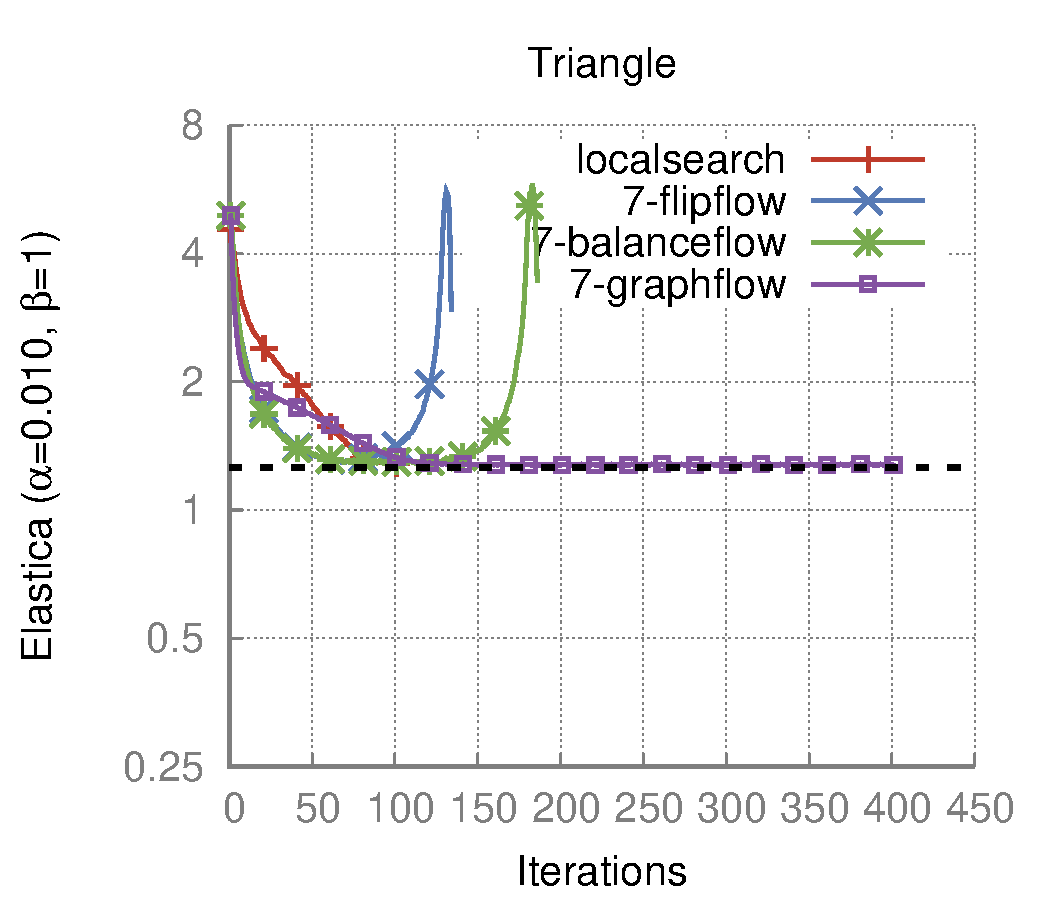
\includegraphics[scale=0.45]{figures/chapter9/free-elastica/plots/iteration/main_experiment/len_pen_0.01/radius-7/triangle.pdf} &
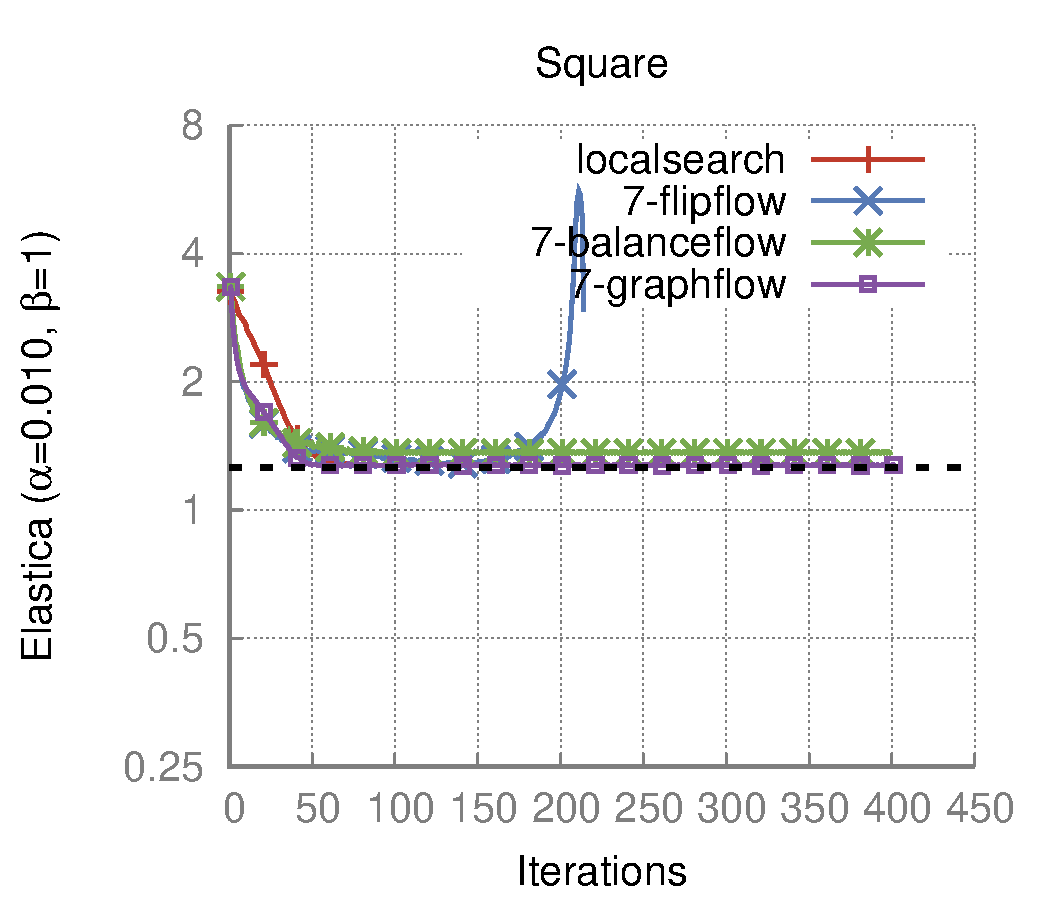
\includegraphics[scale=0.45]{figures/chapter9/free-elastica/plots/iteration/main_experiment/len_pen_0.01/radius-7/square.pdf}\\[1em]
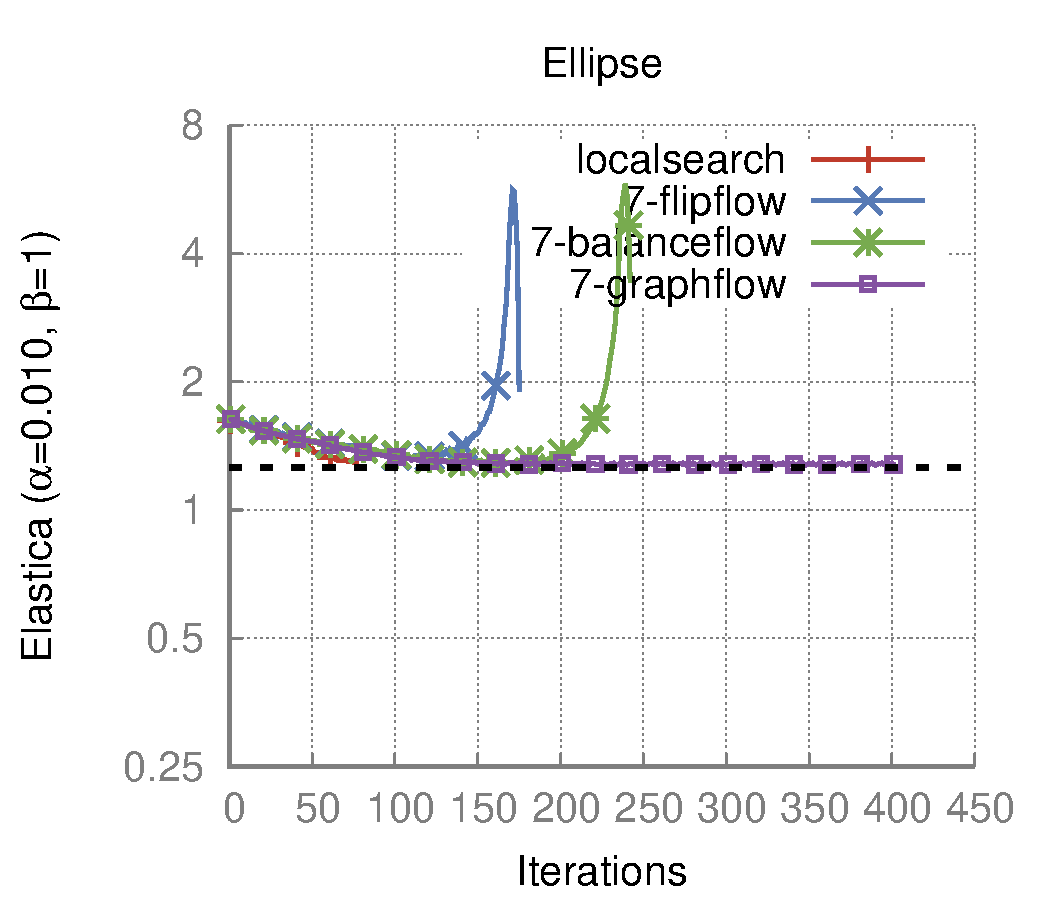
\includegraphics[scale=0.45]{figures/chapter9/free-elastica/plots/iteration/main_experiment/len_pen_0.01/radius-7/ellipse.pdf} &
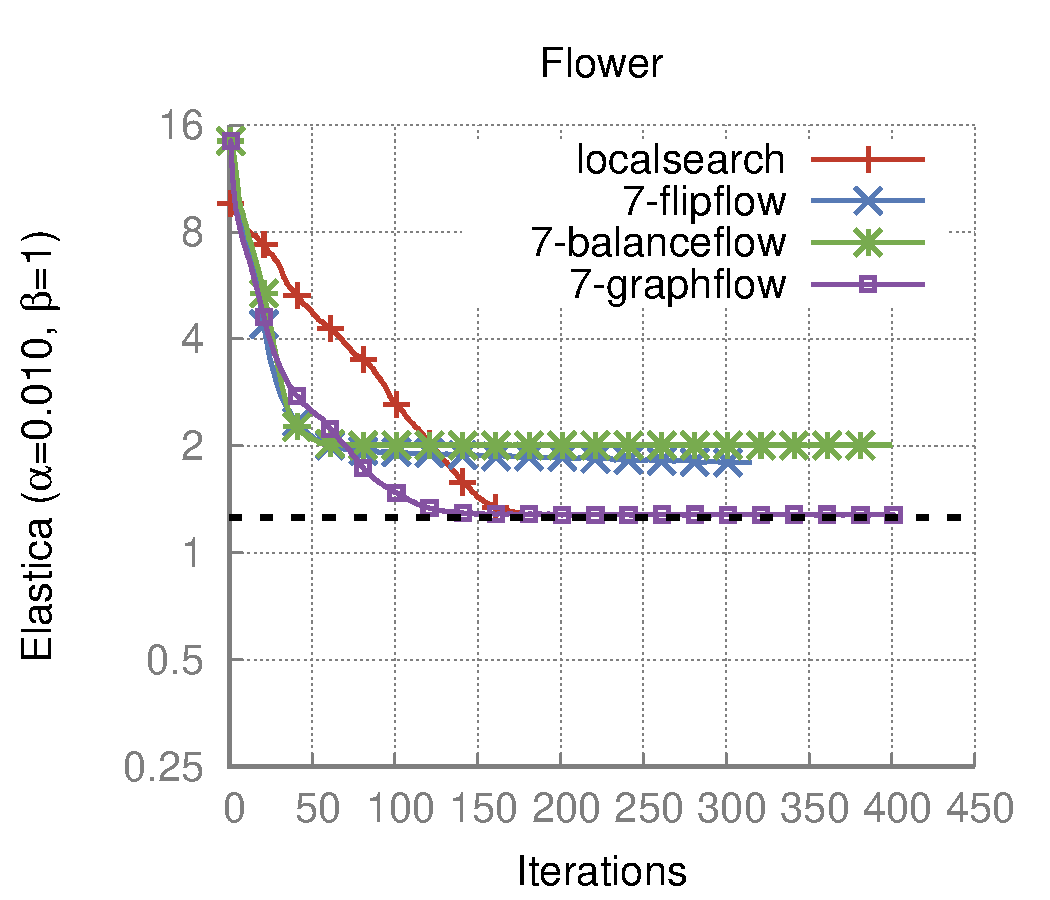
\includegraphics[scale=0.45]{figures/chapter9/free-elastica/plots/iteration/main_experiment/len_pen_0.01/radius-7/flower.pdf}\\[1em]
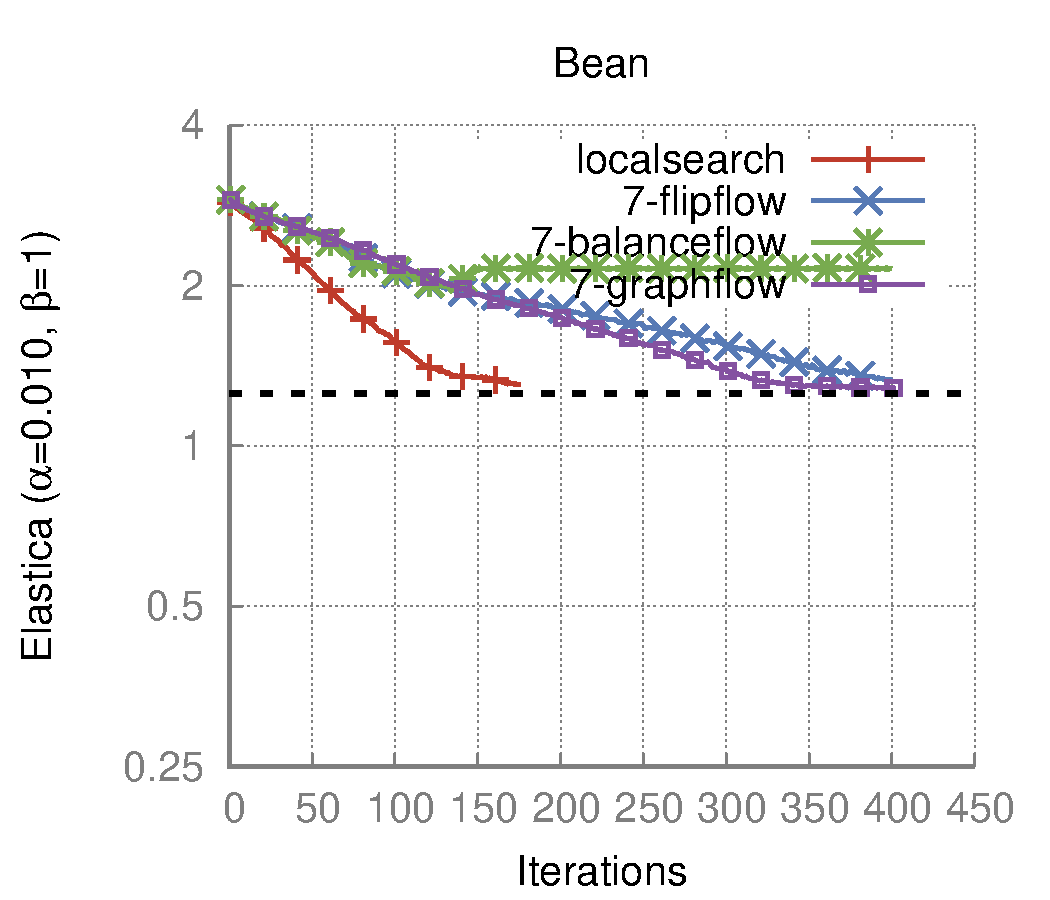
\includegraphics[scale=0.45]{figures/chapter9/free-elastica/plots/iteration/main_experiment/len_pen_0.01/radius-7/bean.pdf}
\end{tabular}
\caption{Digital Elastica value evolution per iteration of the General experiment for the free Elastica.}
\label{fig:plots-free-elastica-general}
\end{figure}

\subsection{Radius choice}

In the Radius-choice experiment, we set the length penalization parameter to $\alpha=0.001$. Compared to the General experiment, the expected behaviour is that the shapes will grow till reach the optimal disk of radius $1/0.001^{0.5} \approx 31$. This experiment evidentiates the natural observation that the choice of the $eRadius$ parameter is important to the optimal shape achievement.

In the case of FlipFlow and BalanceFlow, the evolution goes faster with a larger radius, but the shape never grows, it only shrinks. On the other hand, LocalSearch and GraphFlow are sensitive to the value of $\alpha$ and they can grow or shrink the shape acoordingly. Moreover, the choice of $eRadius$ defines how closer the solution will be from the optimum.

We recall that the II estimator measures curvature by using a disk of a given radius. The radius parameter defines the range of values estimated by the estimator. At first glance, a larger radius returns a more precise estimation, but we should be careful in not use a radius larger than the shape reach at the point of estimation.

However, for the Radius-choice experiment, a value $eRadius=7$ is too small to identify the small variations that a shape that grows till become a disk of radius $31$ suffers. Therefore, when we set $eRadius=12$ both LocalSearch and GraphFlow return solutions closer to the optimal as we can check in~\cref{fig:results-free-elastica-radius-choice,fig:plots-free-elastica-radius-choice}.


\begin{figure}
\begin{tabular}{m{1.5cm}cccc}
& LocalSearch & FlipFlow & BalanceFlow & GraphFlow\\[1em]
$r=7$ & \raisebox{-.5\height}{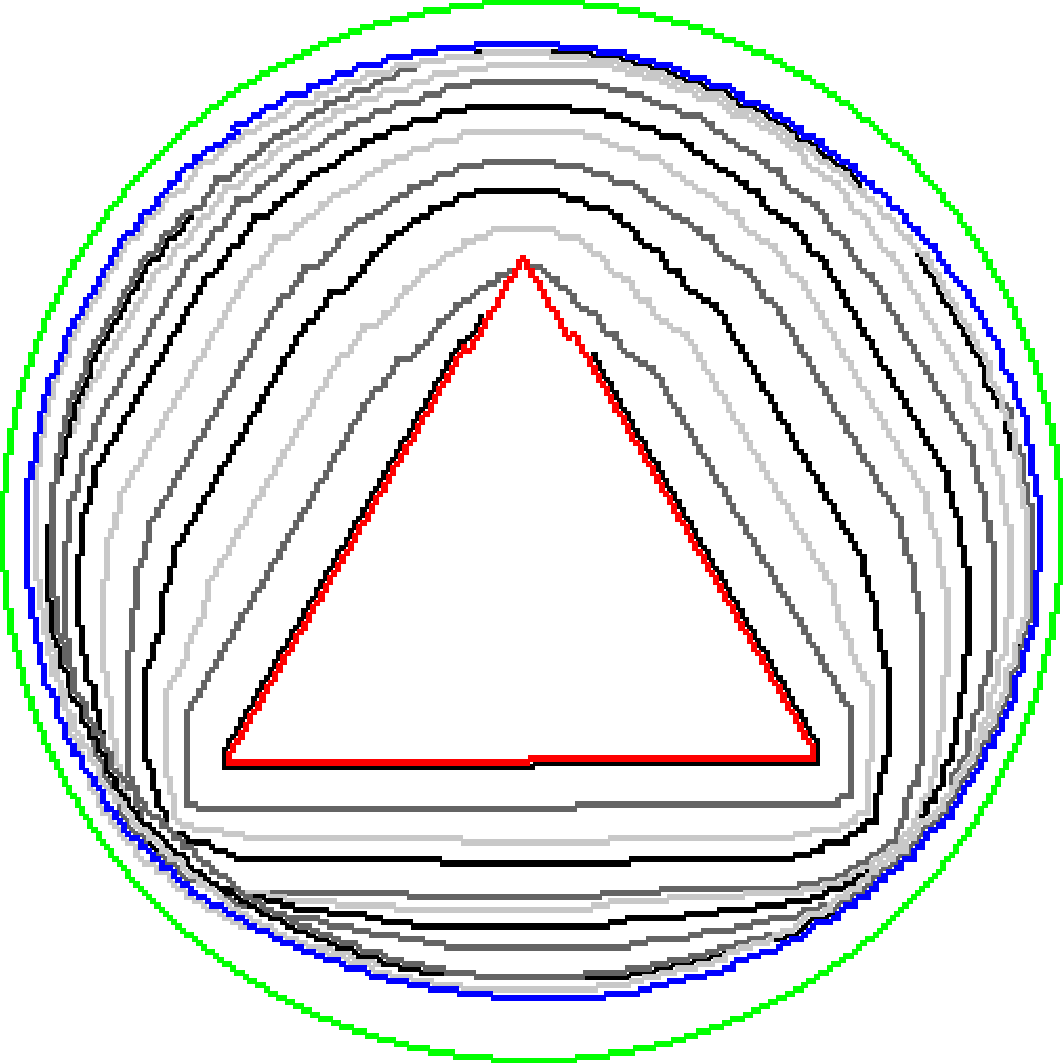
\includegraphics[scale=0.15]{figures/chapter9/free-elastica/localsearch/triangle/len_pen-0.001/radius-7/summary.pdf}} & 
\raisebox{-.5\height}{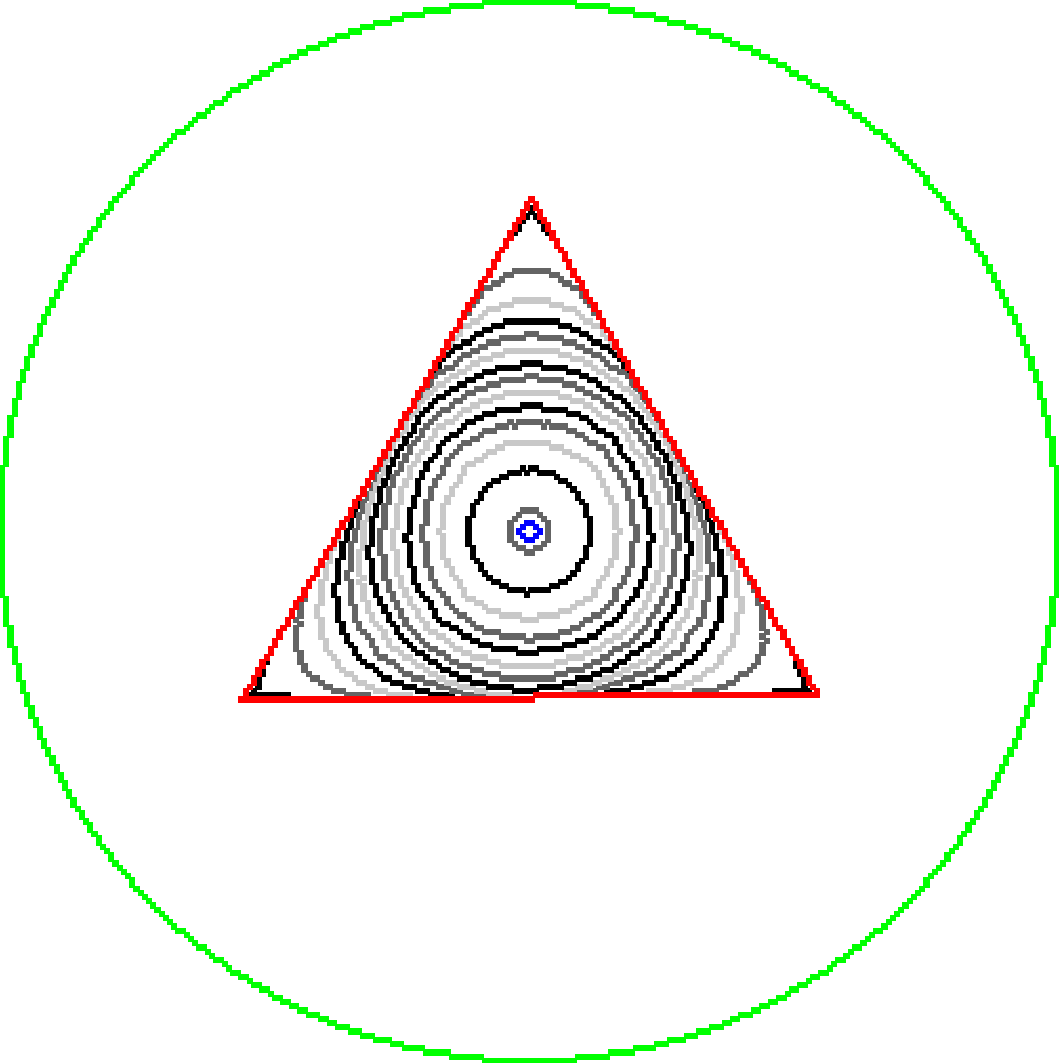
\includegraphics[scale=0.15]{figures/chapter9/free-elastica/flipflow/triangle/len_pen-0.001/radius-7/summary.pdf}} &
\raisebox{-.5\height}{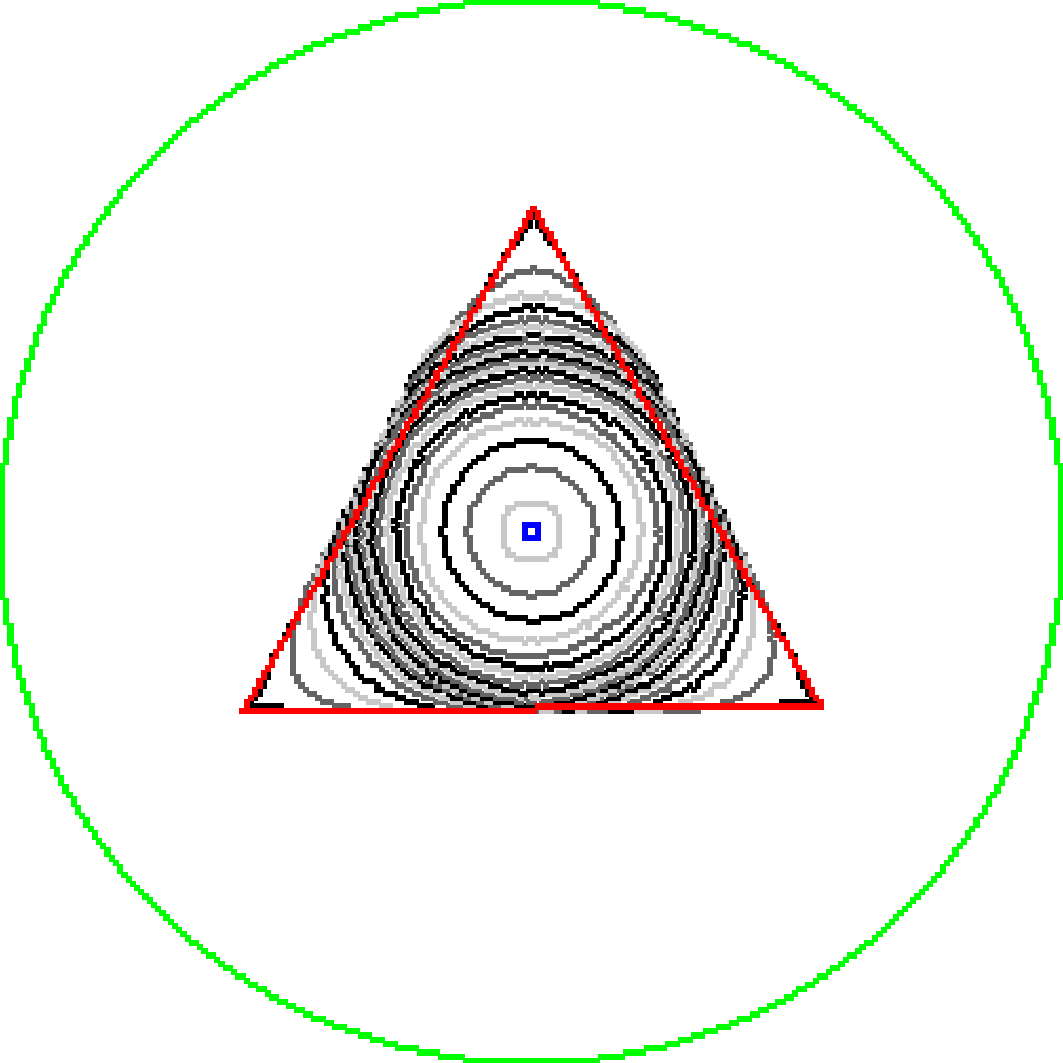
\includegraphics[scale=0.15]{figures/chapter9/free-elastica/balanceflow/triangle/len_pen-0.001/radius-7/summary.pdf}} &
\raisebox{-.5\height}{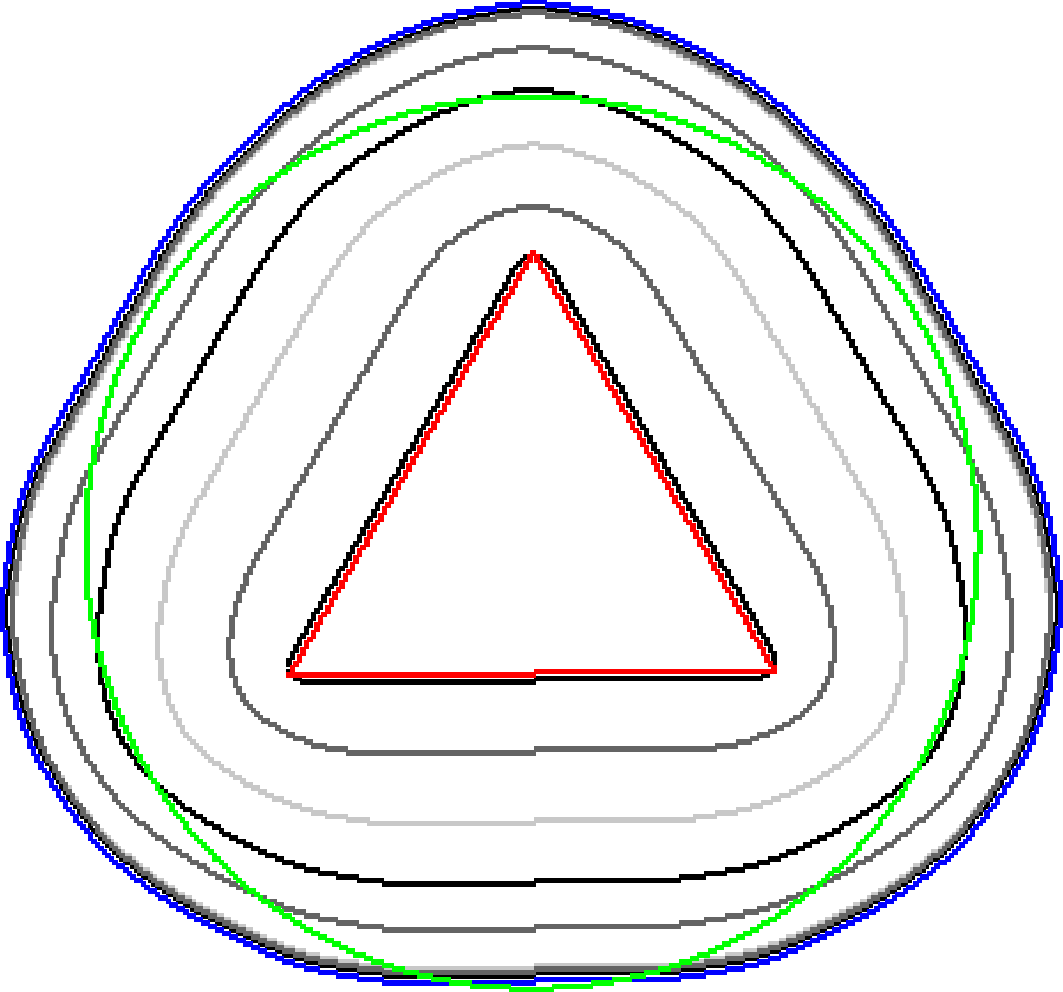
\includegraphics[scale=0.15]{figures/chapter9/free-elastica/graphflow/triangle/len_pen-0.001/radius-7/summary.pdf}} \\[4em]
$r=12$ & \raisebox{-.5\height}{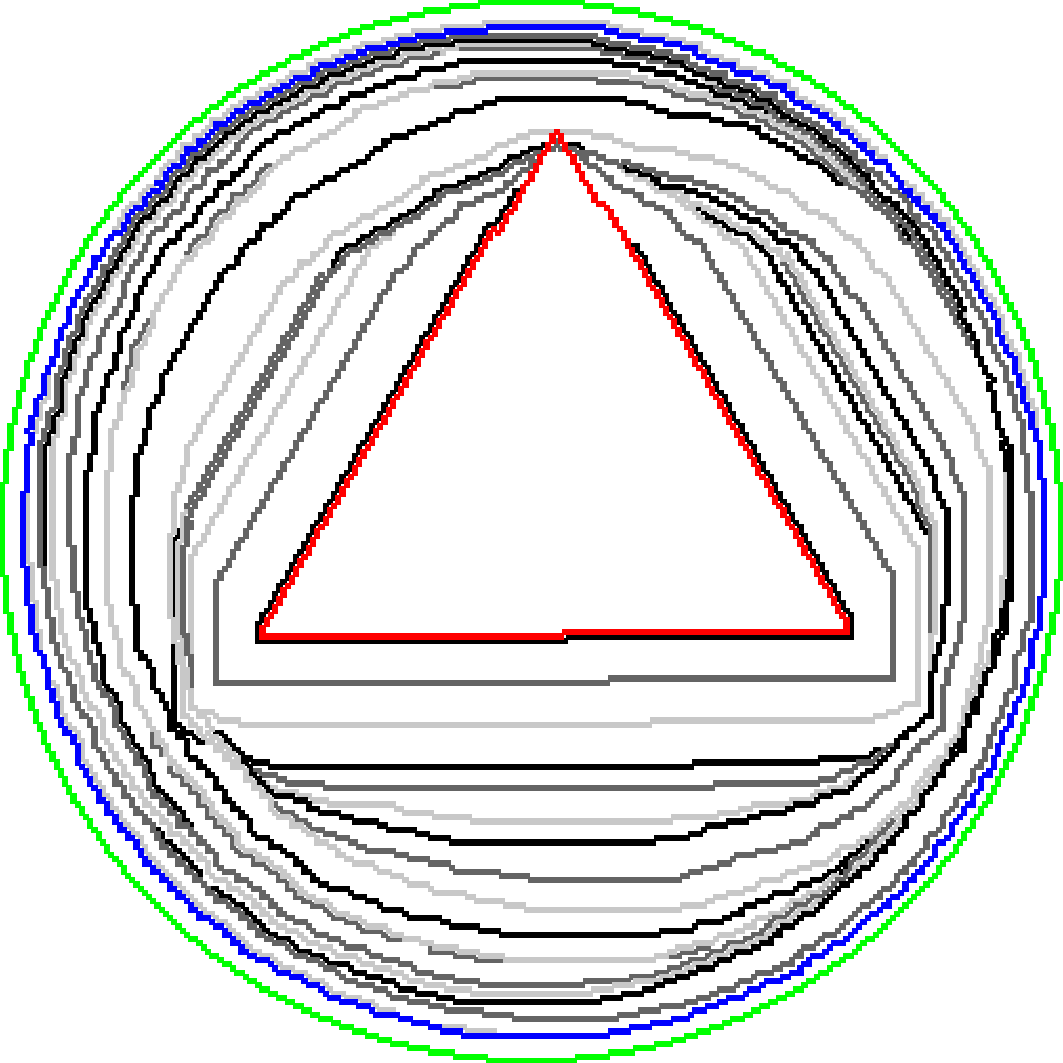
\includegraphics[scale=0.15]{figures/chapter9/free-elastica/localsearch/triangle/len_pen-0.001/radius-12/summary.pdf}} & 
\raisebox{-.5\height}{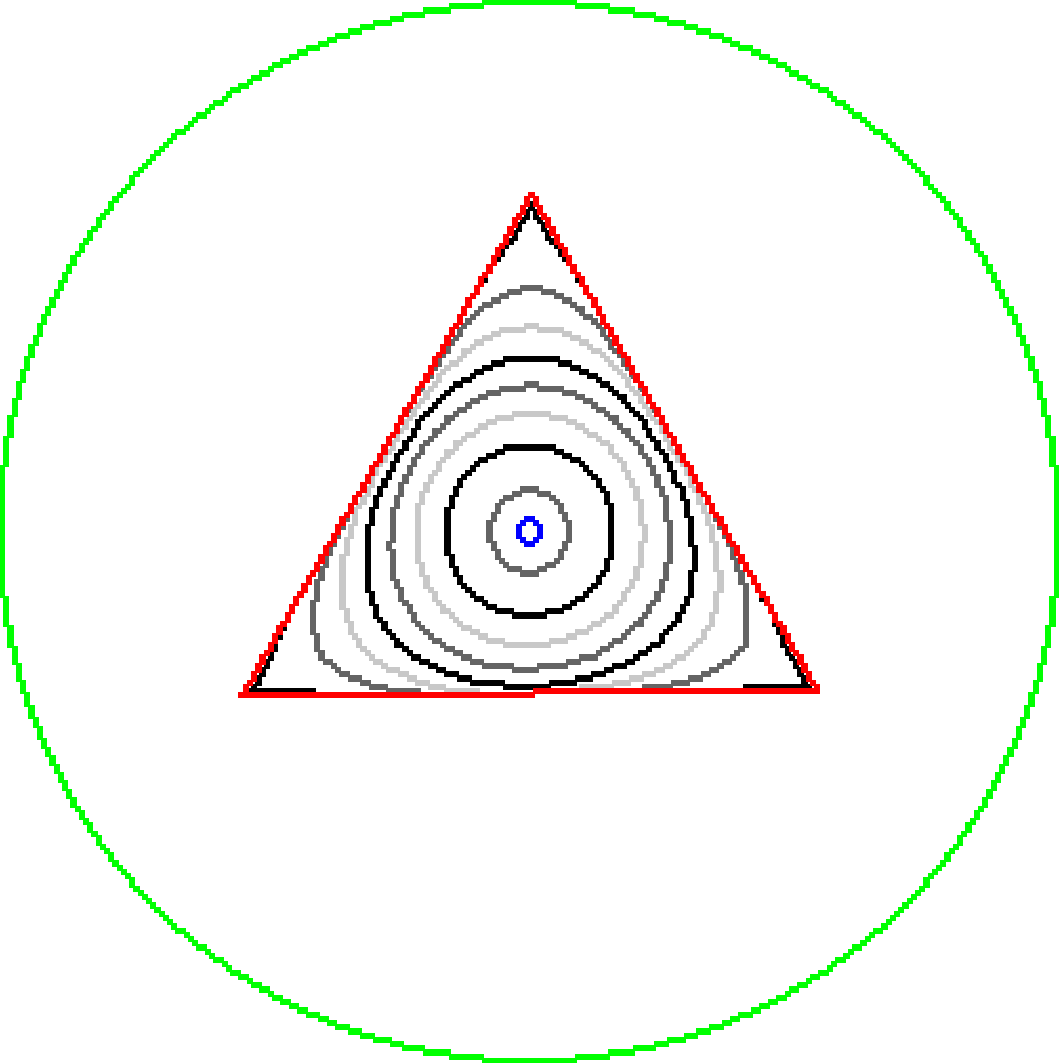
\includegraphics[scale=0.15]{figures/chapter9/free-elastica/flipflow/triangle/len_pen-0.001/radius-12/summary.pdf}} &
\raisebox{-.5\height}{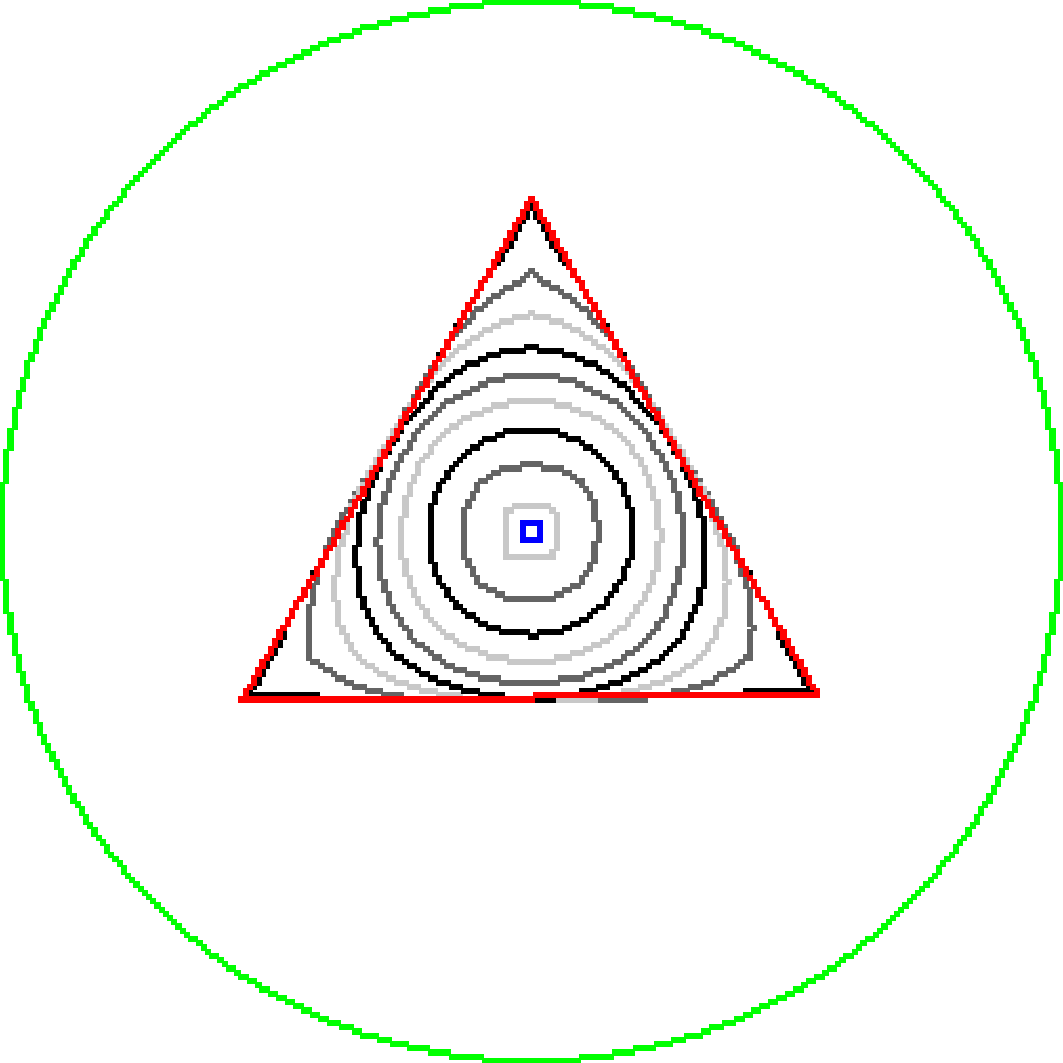
\includegraphics[scale=0.15]{figures/chapter9/free-elastica/balanceflow/triangle/len_pen-0.001/radius-12/summary.pdf}} &
\raisebox{-.5\height}{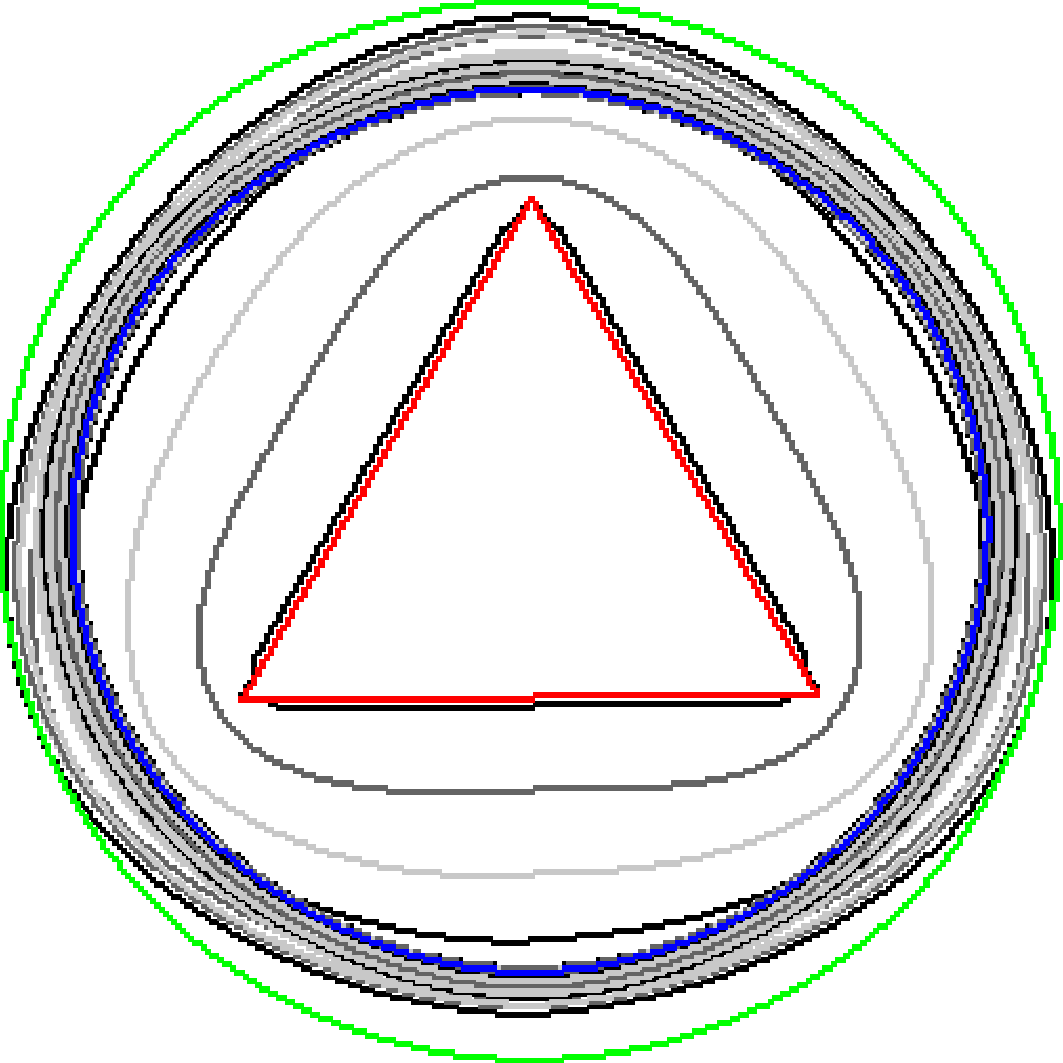
\includegraphics[scale=0.15]{figures/chapter9/free-elastica/graphflow/triangle/len_pen-0.001/radius-12/summary.pdf}} \\[4em]
$r=7$ & \raisebox{-.5\height}{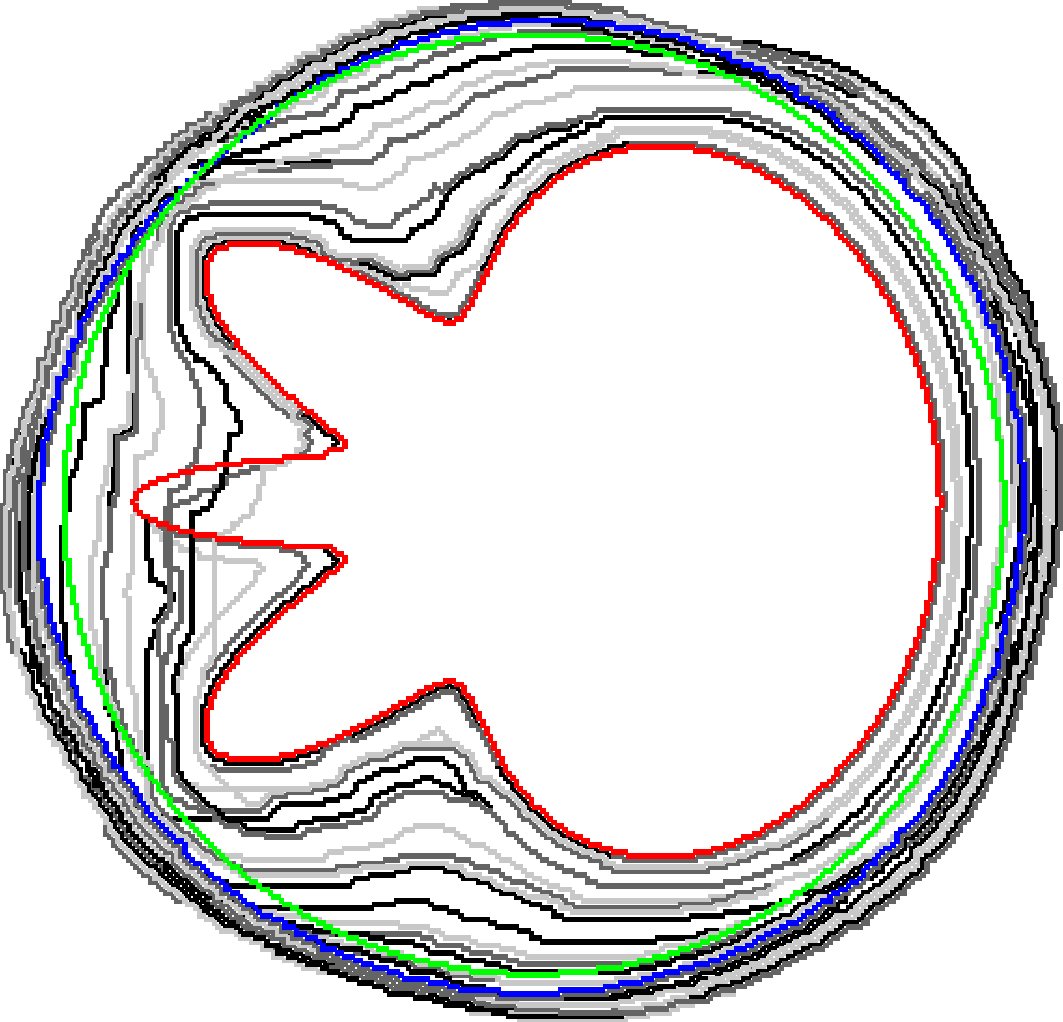
\includegraphics[scale=0.15]{figures/chapter9/free-elastica/localsearch/flower/len_pen-0.001/radius-7/summary.pdf}} & 
\raisebox{-.5\height}{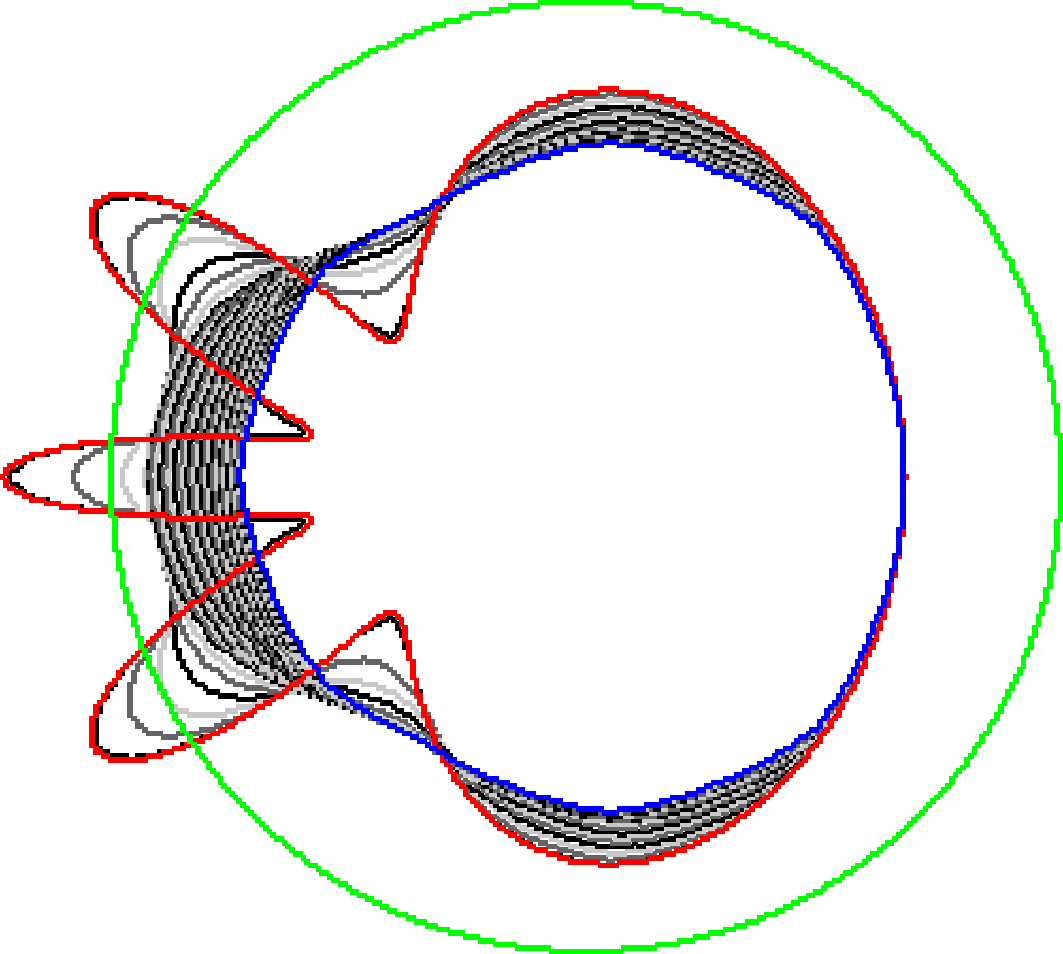
\includegraphics[scale=0.15]{figures/chapter9/free-elastica/flipflow/flower/len_pen-0.001/radius-7/summary.pdf}} &
\raisebox{-.5\height}{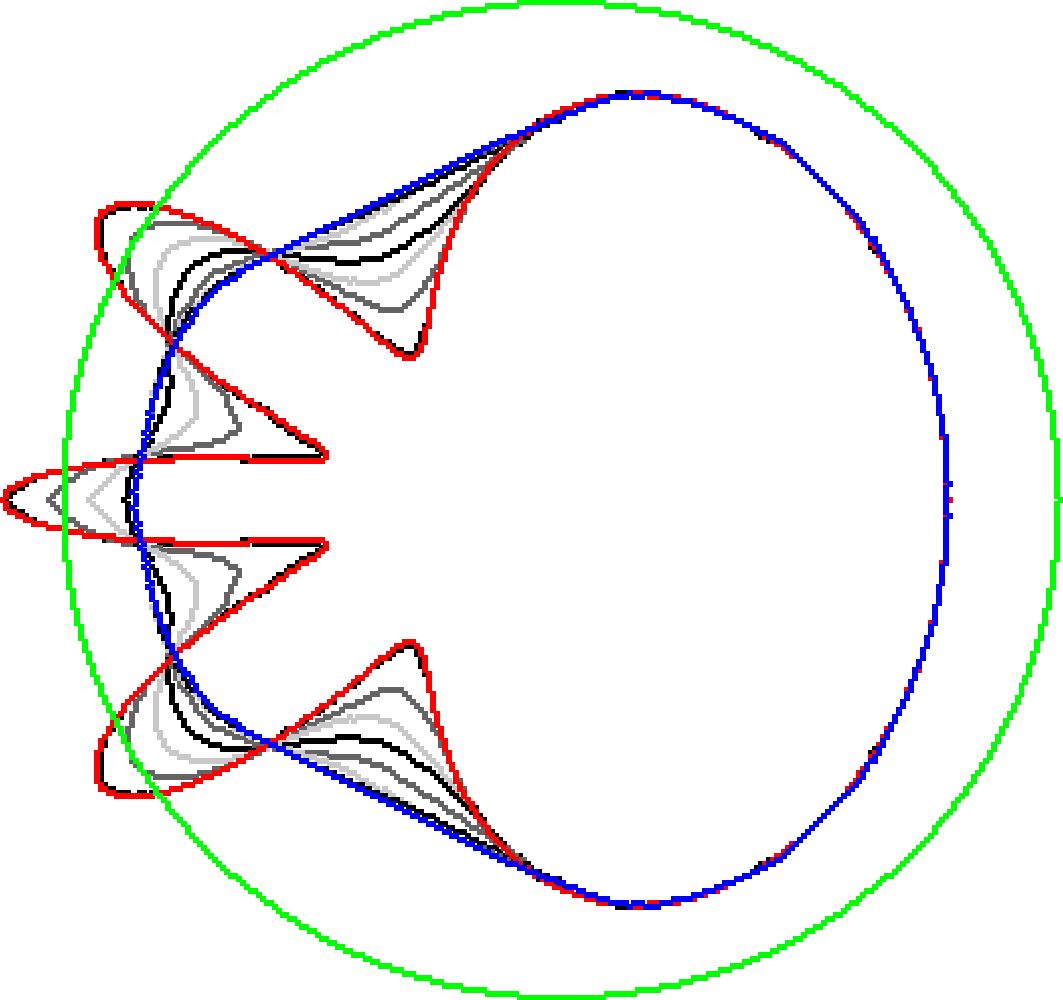
\includegraphics[scale=0.15]{figures/chapter9/free-elastica/balanceflow/flower/len_pen-0.001/radius-7/summary.pdf}} &
\raisebox{-.5\height}{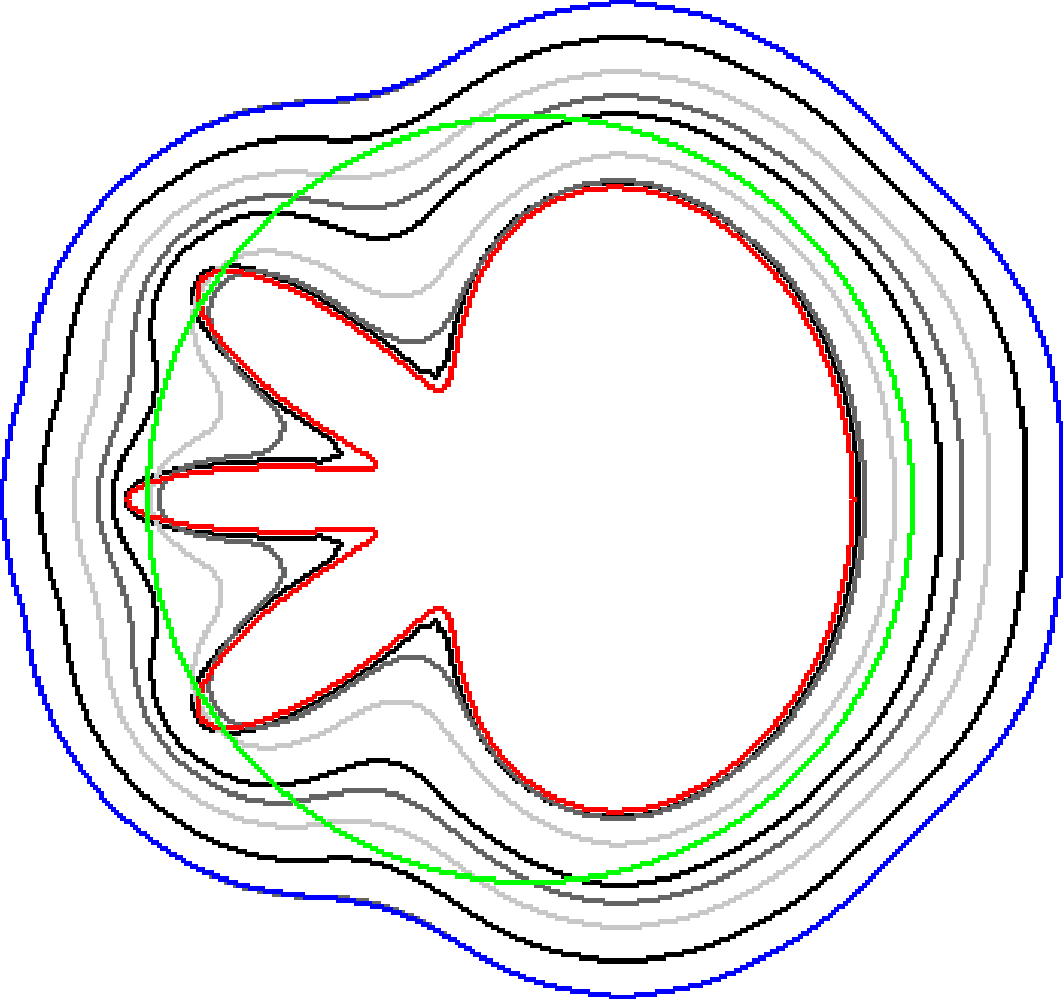
\includegraphics[scale=0.15]{figures/chapter9/free-elastica/graphflow/flower/len_pen-0.001/radius-7/summary.pdf}} \\[4em]
$r=12$ & \raisebox{-.5\height}{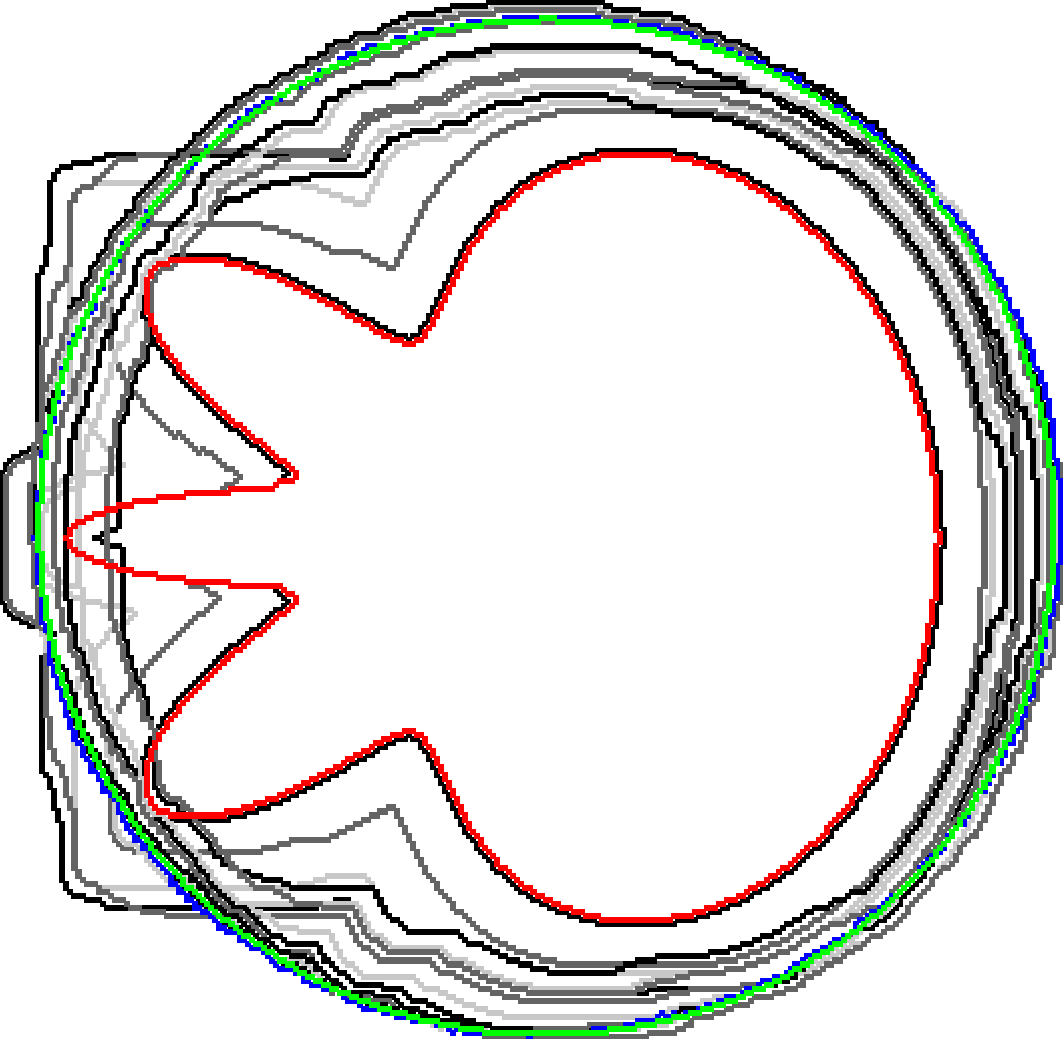
\includegraphics[scale=0.15]{figures/chapter9/free-elastica/localsearch/flower/len_pen-0.001/radius-12/summary.pdf}} & 
\raisebox{-.5\height}{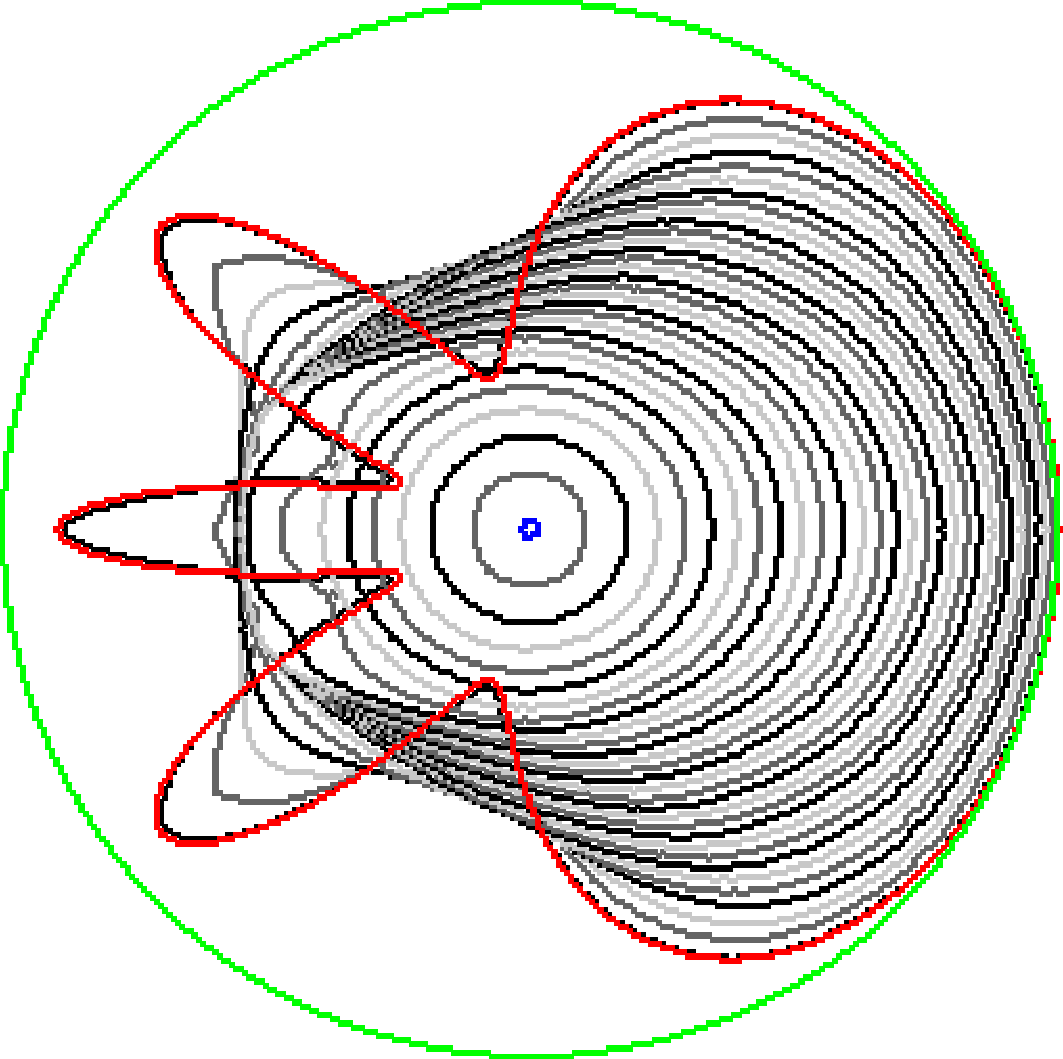
\includegraphics[scale=0.15]{figures/chapter9/free-elastica/flipflow/flower/len_pen-0.001/radius-12/summary.pdf}} &
\raisebox{-.5\height}{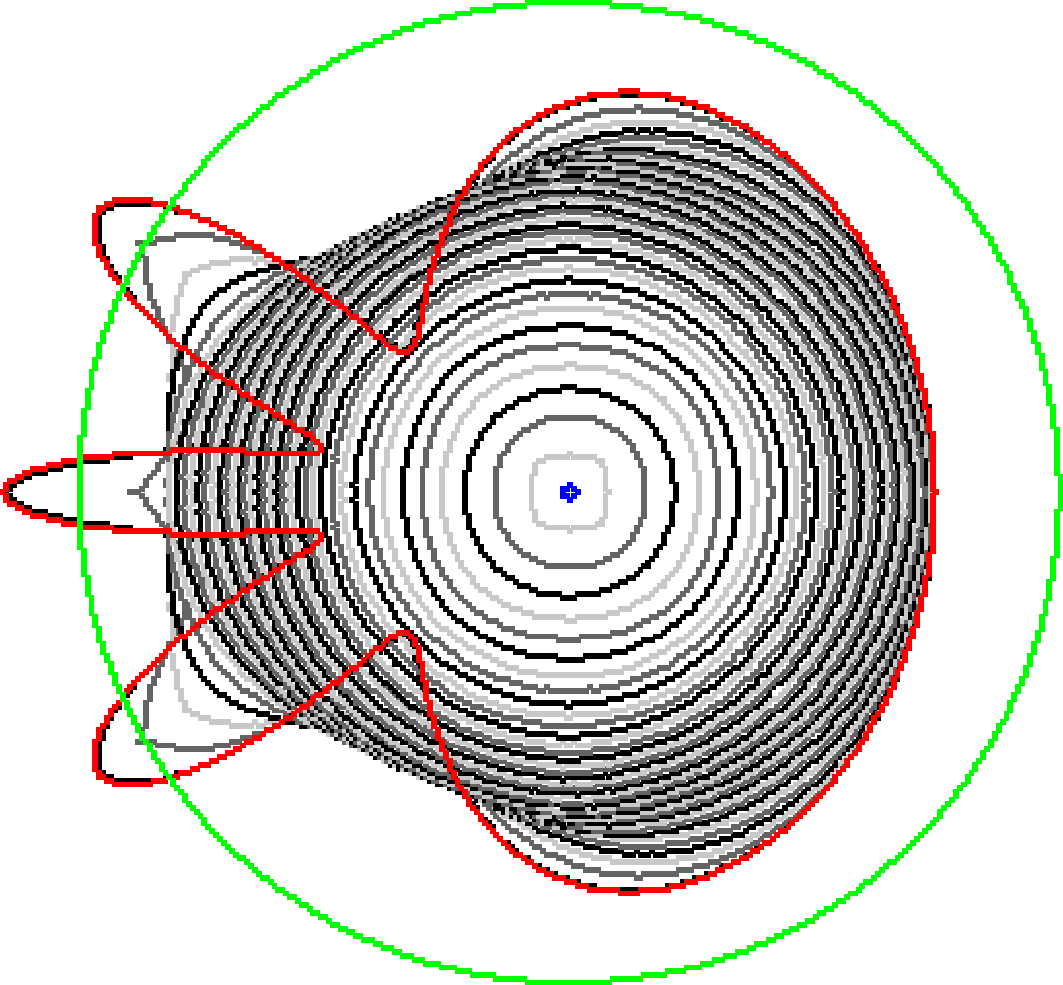
\includegraphics[scale=0.15]{figures/chapter9/free-elastica/balanceflow/flower/len_pen-0.001/radius-12/summary.pdf}} &
\raisebox{-.5\height}{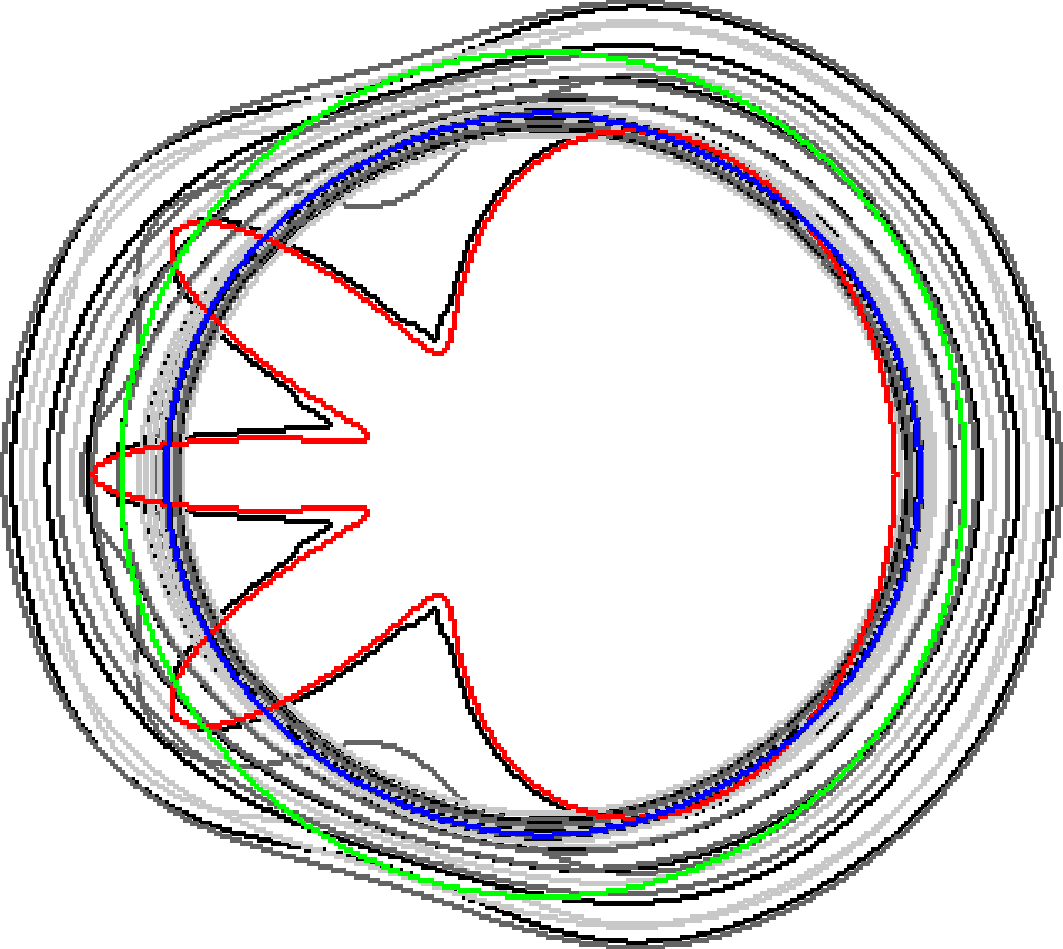
\includegraphics[scale=0.15]{figures/chapter9/free-elastica/graphflow/flower/len_pen-0.001/radius-12/summary.pdf}}
\end{tabular}
\caption{Evolutions of the Radius-choice experiment for the free Elastica.}
\label{fig:results-free-elastica-radius-choice}
\end{figure}

\begin{figure}
\begin{tabular}{cc}
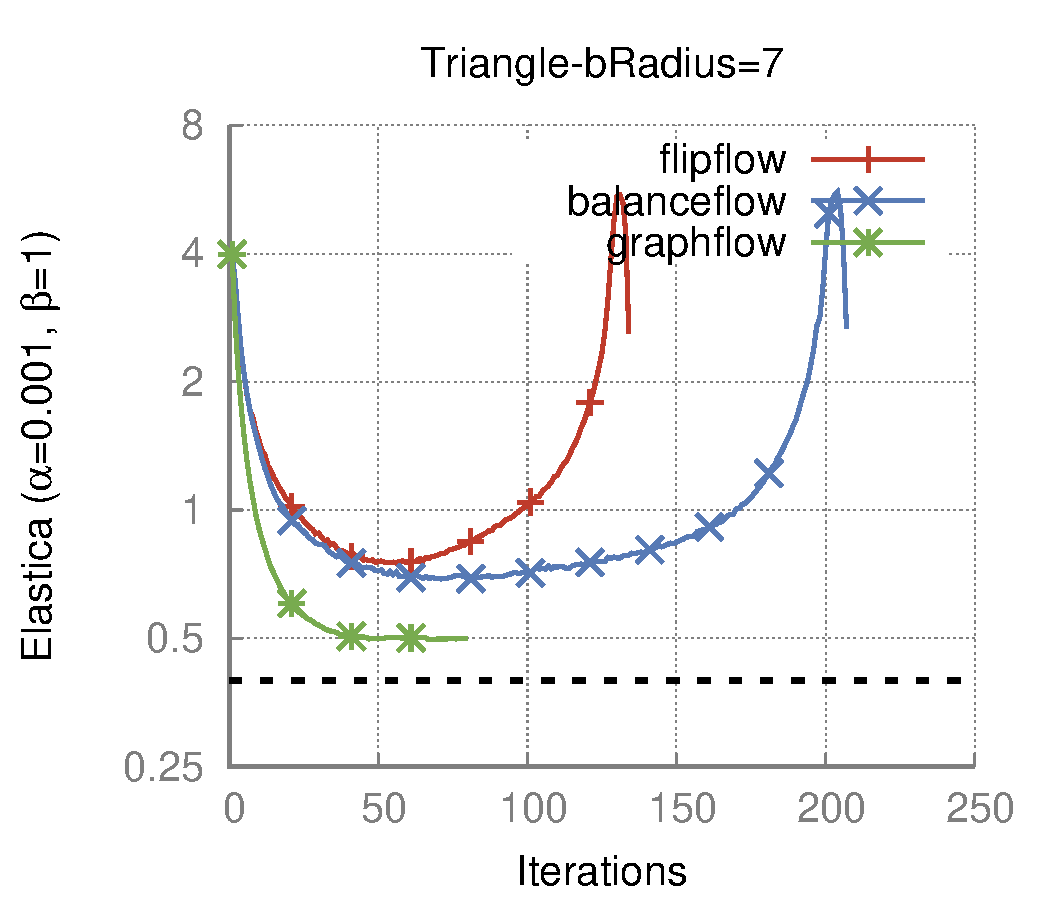
\includegraphics[scale=0.4]{figures/chapter9/free-elastica/plots/iteration/radius_choice/len_pen_0.001/radius-7/triangle.pdf} & 
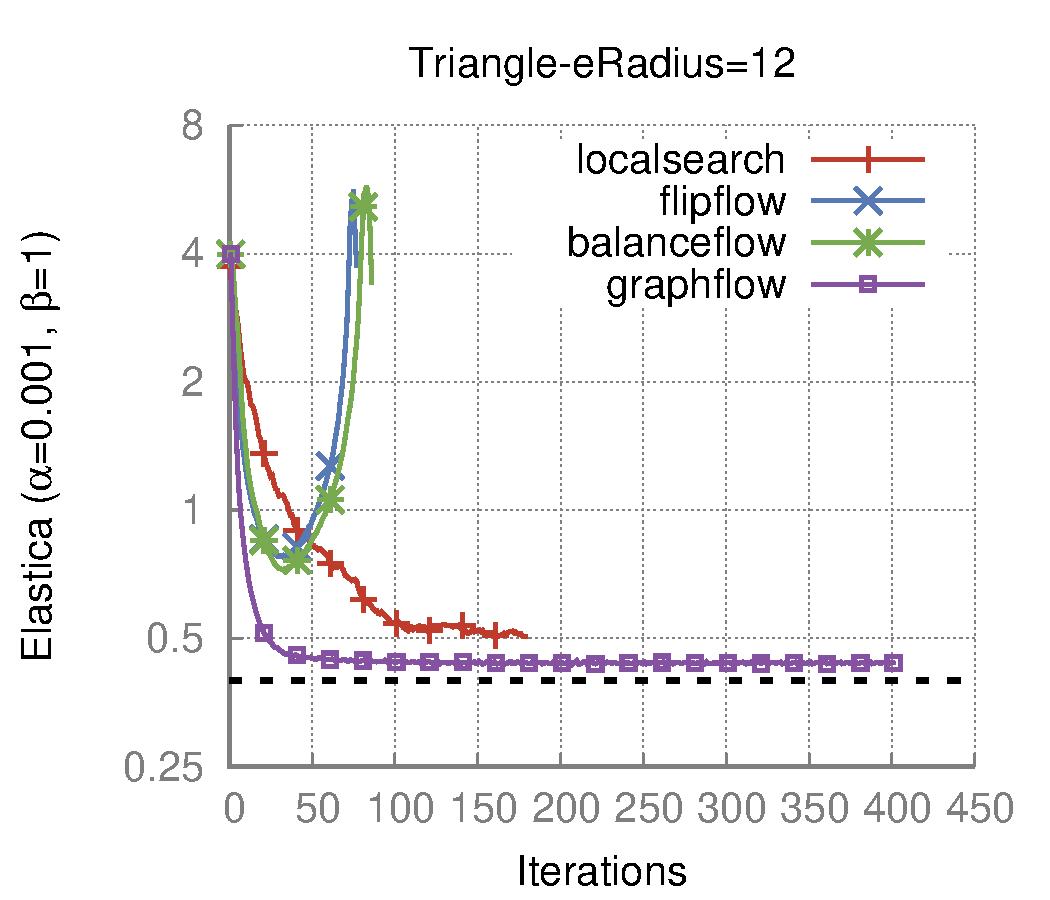
\includegraphics[scale=0.4]{figures/chapter9/free-elastica/plots/iteration/radius_choice/len_pen_0.001/radius-12/triangle.pdf}\\[1em] 
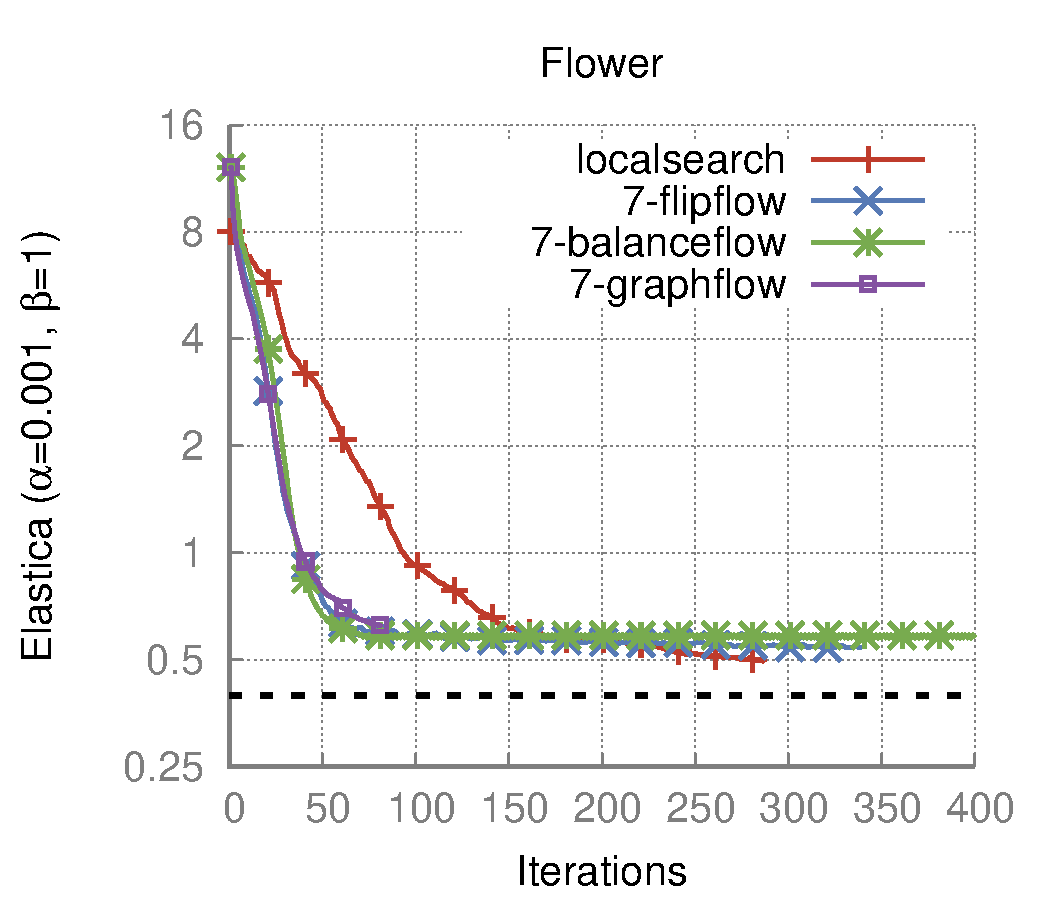
\includegraphics[scale=0.4]{figures/chapter9/free-elastica/plots/iteration/radius_choice/len_pen_0.001/radius-7/flower.pdf} & 
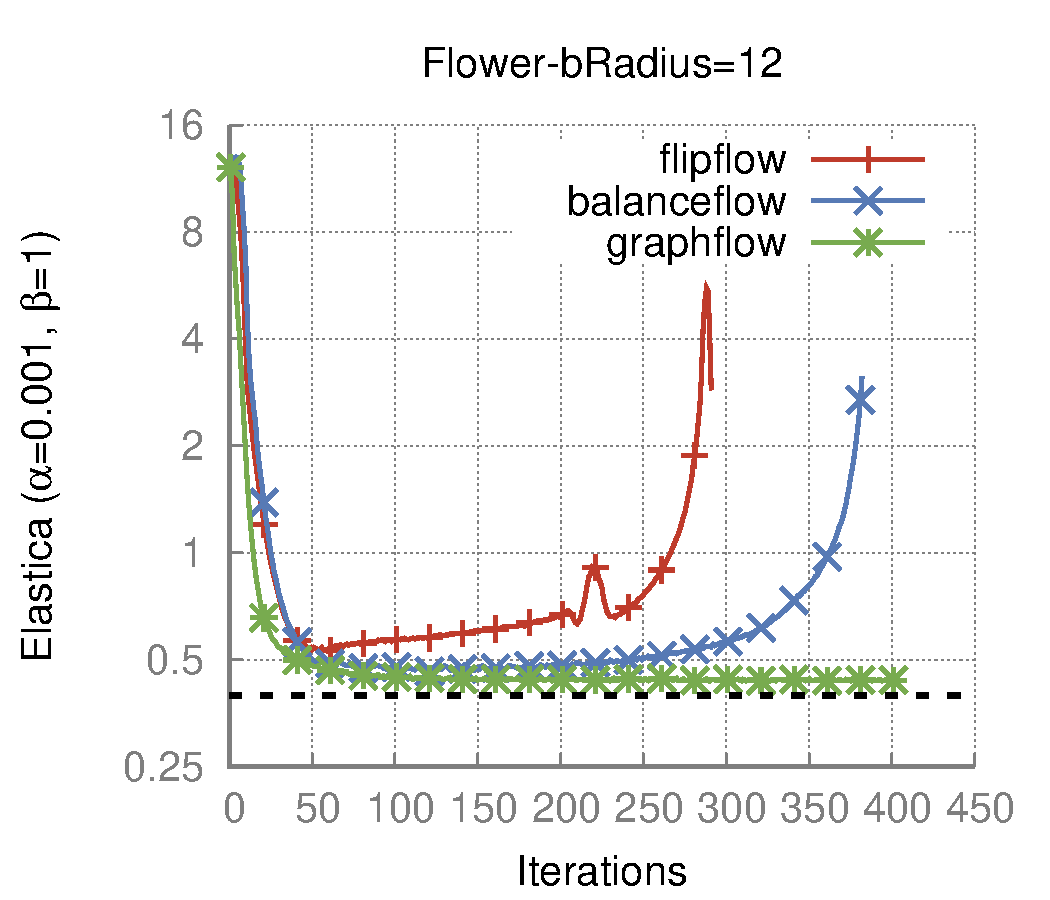
\includegraphics[scale=0.4]{figures/chapter9/free-elastica/plots/iteration/radius_choice/len_pen_0.001/radius-12/flower.pdf}
\end{tabular}
\caption{Digital Elastica value evolution per iteration of the Radius-choice experiment for the free Elastica.}
\label{fig:plots-free-elastica-radius-choice}
\end{figure}


\section{Constrained Elastica}

The constrained Elastica problem consists in to find the shape of minimum digital Elastica that respects some set of constraints. We approach the problem by iteractively evolving some initial shape. We realized experiments with two different set of constraints. In the first, we impose that a set of pixels in the digital boundary of the initial shape must persist in the final shape. In the second, we evolve a curve, instead of a shape, which the endpoints are fixed. 

For the constrained Elastica, only LocalSearch and GraphFlow were evaluated. The FlipFlow and BalanceFlow can be modified to evolve the constrained Elastica, but its implementation is tiresome and we believe the results will not be better than those given by LocalSearch and GraphFlow. Moreover, for a $0$-neighborhood, the GraphFlow behaves very similarly to FlipFlow and BalanceFlow.

\subsection{General experiment}

\subsection{Radius choice}

\begin{table}
\centering
\begin{tabular}{|c|c|c|c|c|c|c|c|c|}
\cline{7-9}
\multicolumn{6}{c|}{} & $LS$ & \multicolumn{2}{|c|}{$GF$}\\
\hline
Experiment & $maxIt$ & $vRadius$ & $eRadius$ & $\alpha$ & $\beta$  & $nc$ & $a$ & $ob$ \\
\hline
General & $400$ & $5$ & $7$ & $0.01$ & $1$  & $4$  & $2$ & $3$ \\
\hline
\multirow{2}{*}{Radius-choice} & \multirow{2}{*}{$400$} & \multirow{2}{*}{$5$} & $7$ & \multirow{2}{*}{$0.001$} & \multirow{2}{*}{$1$}  & \multirow{2}{*}{4}  & \multirow{2}{*}{$2$} & \multirow{2}{*}{$3$} \\
& &  & $12$ &  & &  & &  \\
\hline
\end{tabular}
\caption{Parameters listing for the free Elastica experiments. The headers $LS,GF$ highlights parameters that are exclusive for the LocalSearch and GraphFlow models, respectively.}
\label{tab:constrained-elastica-parameters-summary}
\end{table}

\begin{figure}
\center
\captionsetup{type=table}
\begin{tabular}{|l|c|c|c|c|c|}
\hline
& Pixels & LocalSearch & GraphFlow \\
\hline
Curve-1 & 8315 & 1.7s/it & 0.14s/it\\
Curve-2 & 12769 & 1s/it & 0.12s/it\\
Flower-1  & 10038 & 1.3s/it & 0.1s/it \\
Flower-2 & 26321 & 4.7s/it & 0.14s/it\\
\hline
\end{tabular}
\caption{Running time and input size of the General experiment for the constrained Elastica.}
\label{tab:rtime-constrained-elastica-general} 
\end{figure}

%The parameters used in the comparison are listed in table~\cref{} and the running times in table~\cref{}. The results are displayed in figures~\cref{} and~\cref{}, one for each value of $\alpha$. 

The LocalSearch approach behaves as expected in both experiments, both the GraphFlow encounters some difficults to evolve in the case of fixed endpoint orientations. We recall that the GraphFlow uses as neighborhood a set of dilations and erosions of the initial shape. Instead, if we use a neighborhood in which just some pixels of the inner or outer boundary are changed (in a similar fashion of what is done in the LocalSearch neighborhood, but with fewer members) we believe that we can recover better results.

\section{Image segmentation}

The FlipFlow,BalanceFlow and GraphFlow can be extended to do image segmentation. In this section we show the results of several experiments that illustrates the influence of the weight parameters (length,curvature,data) in the final segmentation. At the last section we compare our results with the Schoenemann linear curvature regularization (SLCR). 

All three models (FF,BF,GF) need a initial segmentation as input. This segmentation is given by a single iteration of the Grabcut algorithm.~\cref{tab:image-segmentation-parameters-summary} lists the parameters configuration for each experiment and~\cref{tab:rtime-image-segmentation-general} summarizes their running times. 

We categorize the experiments in two sections. In the first, we study the influence of eqch parameter in the produced segmentation and in the second we compare our segmentations with those produced by SLCR.


\begin{table}
\centering
\begin{tabular}{|c|c|c|c|c|c|c|c|c|c|c|c|}
\cline{7-12}
\multicolumn{6}{c|}{} & \multicolumn{2}{|c|}{$FF,BF$} & \multicolumn{4}{|c|}{$GF$}\\
\hline
Experiment & $maxIt$ & $vRadius$ & $eRadius$ & $\alpha$ & $\beta$  & $\gamma$ & $d$ & $a$ & $ob$ & $\lambda_r$ & $\lambda_b$ \\
\hline
\multirow{3}{*}{Exp-$\alpha$} & \multirow{3}{*}{$200$} & \multirow{3}{*}{$7$} & \multirow{3}{*}{$7$} & $0$ & \multirow{3}{*}{$0$} & \multirow{3}{*}{$2$} & \multirow{3}{*}{$0$} & \multirow{3}{*}{$2$} & \multirow{3}{*}{$2$} & \multirow{3}{*}{$2$} & \multirow{3}{*}{$2$} \\
&  & & & $0.5$ & & & & & & &\\
&  & & & $1$ & & & & & & &\\
\hline
\multirow{3}{*}{Exp-$\beta$} & \multirow{3}{*}{$200$} & \multirow{3}{*}{$7$} & \multirow{3}{*}{$7$} & \multirow{3}{*}{$0.1$} & $0.1$ & \multirow{3}{*}{$2$} & \multirow{3}{*}{$0$} & \multirow{3}{*}{$2$} & \multirow{3}{*}{$2$} & \multirow{3}{*}{$2$} & \multirow{3}{*}{$2$} \\
&  & & & & $1$ & & & & & &\\
&  & & & & $3$ & & & & & &\\
\hline
\multirow{3}{*}{Exp-$\gamma$} & \multirow{3}{*}{$200$} & \multirow{3}{*}{$7$} & \multirow{3}{*}{$7$} & \multirow{3}{*}{$0.1$} & \multirow{3}{*}{$1$} & $0$ & \multirow{3}{*}{$0$} & \multirow{3}{*}{$2$} & \multirow{3}{*}{$2$} & $0$ & $0$ \\
&  & & & & & $1$ & & & & $1$ & $1$\\
&  & & & & & $5$ & & & & $5$ & $5$\\
\hline
\multirow{3}{*}{Exp-$radius$} & \multirow{3}{*}{$200$} & $3$ & $3$ & \multirow{3}{*}{$0.1$} & \multirow{3}{*}{$1$} & \multirow{3}{*}{$1$} & \multirow{3}{*}{$0$} & \multirow{3}{*}{$2$} & \multirow{3}{*}{$2$} & \multirow{3}{*}{$1$} & \multirow{3}{*}{$1$} \\
&  & $7$ & $7$ & & & & & & & & \\
&  & $12$ & $12$ & & & & & & & & \\
\hline
\end{tabular}
\caption{Parameters listing for the image segmentation experiments. The headers $FF,BF,GF$ highlights parameters that are exclusive for the FlipFLow, BalanceFlow and GraphFlow models, respectively.}
\label{tab:image-segmentation-parameters-summary}
\end{table}

\begin{figure}
\center
\captionsetup{type=table}
\begin{tabular}{|l|c|c|c|}
\hline
& \multicolumn{3}{|c|}{Running time}\\
& Minimum & Maximum & Average \\
\hline
FlipFlow & 0 & 1.7s/it & 0.14s/it\\
BalanceFlow & 0 & 1s/it & 0.12s/it\\
GraphFlow & 0 & 1s/it & 0.12s/it\\
\hline
\end{tabular}
\caption{Running time and input size of Exp-eRadius for the image segmentation problem and $eRadius=7$.}
\label{tab:rtime-image-segmentation-general} 
\end{figure}

\subsection{Parameters influence}
The models offer parameters to control the weight of length $(\alpha)$, curvature $(\beta)$ and data ($\gamma,\lambda _r, \lambda _b$). We recall that FF and BF accept a single regional parameter $\gamma$ for data, while GF accepts $\lambda _r$ to ponderate a regional term and $\lambda _b$ to weight a boundary term. The Grabcut input and its result are shown in~\cref{fig:grabcut-input-image-segmentation}. The results are displayed in~\cref{fig:exp-alpha-image-segmentation,fig:exp-beta-image-segmentation,fig:exp-gamma-image-segmentation,fig:exp-radius-image-segmentation}. 

The FlipFlow and BalanceFlow present similar results for all experiments, as expected. The Exp-$\alpha$ experiment regularizes only length, and we can observe that the segmentations produced by all three models tend to be staircased. 

We remark that there is no length penalization in the cost function of the candidate graph. In the GF model, the length regularization plays a role in the validation function, and its influence is noticed for probe-sets with $a>1$. 

On the other hand, experiment Exp-$\beta$ illustrates how the curvature can be used to produce smoother curves in these models. We recall that the shrink or growing behaviour in the case of the GF is controlled by the value of $\alpha$, which in Exp-$\beta$ is set to $\alpha=0.1$. The FF, and BF can grow in concavities, but it presents a general shrinking behaviour.

Finally, Exp-$\gamma$ illustrates the role of data term in the final segmentation result and Exp-$radius$ the effect of the estimation ball radius. It is clear that all three models regularizes the initial segmentation given by Grabcut with respect to the squared curvature, the regularization amount being parameterized by the relation between the data ($\gamma, \theta_r, \theta_b$) and curvature ($\beta$) weights. The best choice of parameters depends on the object to be segmented.


\begin{figure}
\centering
\begin{tabular}{cc}
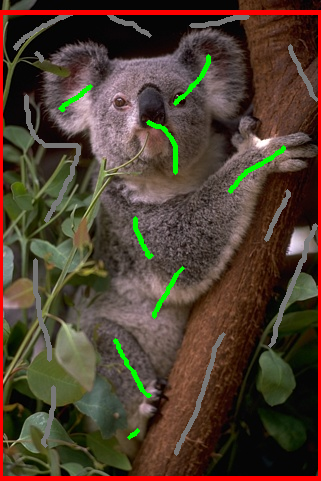
\includegraphics[scale=0.4]{figures/chapter9/segmentation/seeds.png} &
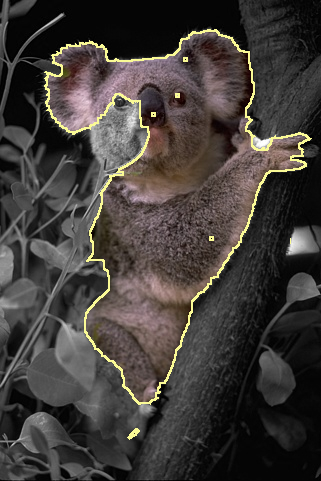
\includegraphics[scale=0.4]{figures/chapter9/segmentation/gc-seg.png}
\end{tabular}
\caption{The Grabcut foreground(blue) and background(seeds) on the left and the resulting segmentation on the right.}
\label{fig:grabcut-input-image-segmentation}
\end{figure}

\begin{figure}
\centering
\begin{tabular}{cccc}
& FlipFlow & BalanceFlow & GraphFlow\\
$\alpha=0.0$ & \raisebox{-.5\height}{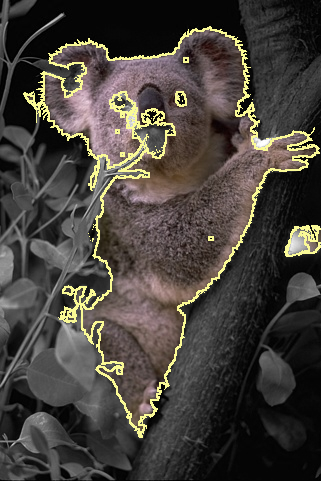
\includegraphics[scale=0.4]{figures/chapter9/segmentation/exp-alpha/flipseg/dalpha-False/neigh-0/alpha-0.0/beta-0.0/lb-2.0/lr-2.0/coala/corrected_seg.png}} &
\raisebox{-.5\height}{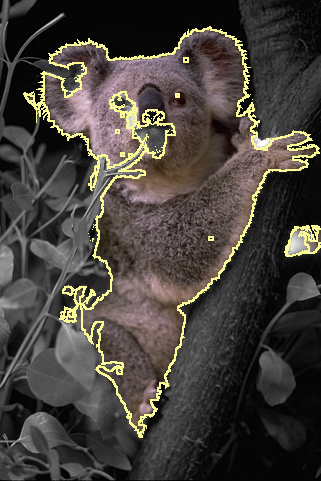
\includegraphics[scale=0.4]{figures/chapter9/segmentation/exp-alpha/balanceseg/dalpha-False/neigh-0/alpha-0.0/beta-0.0/lb-2.0/lr-2.0/coala/corrected_seg.png}} &
\raisebox{-.5\height}{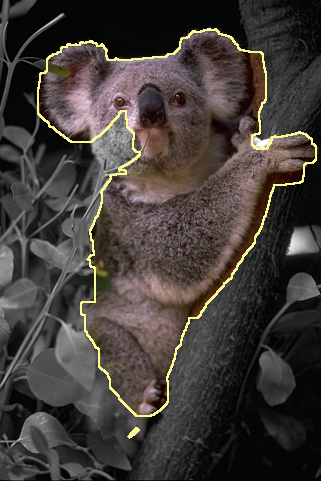
\includegraphics[scale=0.4]{figures/chapter9/segmentation/exp-alpha/graphseg/dalpha-False/neigh-2/alpha-0.0/beta-0.0/lb-2.0/lr-2.0/coala/corrected_seg.png}}\\[10em]

$\alpha=0.5$ & \raisebox{-.5\height}{\includegraphics[scale=0.4]{figures/chapter9/segmentation/exp-alpha/flipseg/dalpha-False/neigh-0/alpha-0.5/beta-0.0/lb-2.0/lr-2.0/coala/corrected_seg.png}} &
\raisebox{-.5\height}{\includegraphics[scale=0.4]{figures/chapter9/segmentation/exp-alpha/balanceseg/dalpha-False/neigh-0/alpha-0.5/beta-0.0/lb-2.0/lr-2.0/coala/corrected_seg.png}} &
\raisebox{-.5\height}{\includegraphics[scale=0.4]{figures/chapter9/segmentation/exp-alpha/graphseg/dalpha-False/neigh-2/alpha-0.5/beta-0.0/lb-2.0/lr-2.0/coala/corrected_seg.png}}\\[10em]

$\alpha=1.0$ & \raisebox{-.5\height}{\includegraphics[scale=0.4]{figures/chapter9/segmentation/exp-alpha/flipseg/dalpha-False/neigh-0/alpha-1.0/beta-0.0/lb-2.0/lr-2.0/coala/corrected_seg.png}} &
\raisebox{-.5\height}{\includegraphics[scale=0.4]{figures/chapter9/segmentation/exp-alpha/balanceseg/dalpha-False/neigh-0/alpha-1.0/beta-0.0/lb-2.0/lr-2.0/coala/corrected_seg.png}} &
\raisebox{-.5\height}{\includegraphics[scale=0.4]{figures/chapter9/segmentation/exp-alpha/graphseg/dalpha-False/neigh-2/alpha-1.0/beta-0.0/lb-2.0/lr-2.0/coala/corrected_seg.png}}
\end{tabular}
\caption{Exp-$\alpha$}
\label{fig:exp-alpha-image-segmentation}
\end{figure}

\begin{figure}
\begin{tabular}{cccc}
& FlipFlow & BalanceFlow & GraphFlow\\
$\beta=0.1$ & \raisebox{-.5\height}{\includegraphics[scale=0.4]{figures/chapter9/segmentation/exp-beta/flipseg/dalpha-False/neigh-0/alpha-0.1/beta-0.1/lb-2.0/lr-2.0/coala/corrected_seg.png}} &
\raisebox{-.5\height}{\includegraphics[scale=0.4]{figures/chapter9/segmentation/exp-beta/balanceseg/dalpha-False/neigh-0/alpha-0.1/beta-0.1/lb-2.0/lr-2.0/coala/corrected_seg.png}} &
\raisebox{-.5\height}{\includegraphics[scale=0.4]{figures/chapter9/segmentation/exp-beta/graphseg/dalpha-False/neigh-2/alpha-0.1/beta-0.1/lb-2.0/lr-2.0/coala/corrected_seg.png}}\\[10em]

$\beta=1$ & \raisebox{-.5\height}{\includegraphics[scale=0.4]{figures/chapter9/segmentation/exp-beta/flipseg/dalpha-False/neigh-0/alpha-0.1/beta-1.0/lb-2.0/lr-2.0/coala/corrected_seg.png}} &
\raisebox{-.5\height}{\includegraphics[scale=0.4]{figures/chapter9/segmentation/exp-beta/balanceseg/dalpha-False/neigh-0/alpha-0.1/beta-1.0/lb-2.0/lr-2.0/coala/corrected_seg.png}} &
\raisebox{-.5\height}{\includegraphics[scale=0.4]{figures/chapter9/segmentation/exp-beta/graphseg/dalpha-False/neigh-2/alpha-0.1/beta-1.0/lb-2.0/lr-2.0/coala/corrected_seg.png}}\\[10em]

$\beta=2$ & \raisebox{-.5\height}{\includegraphics[scale=0.4]{figures/chapter9/segmentation/exp-beta/flipseg/dalpha-False/neigh-0/alpha-0.1/beta-3.0/lb-2.0/lr-2.0/coala/corrected_seg.png}} &
\raisebox{-.5\height}{\includegraphics[scale=0.4]{figures/chapter9/segmentation/exp-beta/balanceseg/dalpha-False/neigh-0/alpha-0.1/beta-3.0/lb-2.0/lr-2.0/coala/corrected_seg.png}} &
\raisebox{-.5\height}{\includegraphics[scale=0.4]{figures/chapter9/segmentation/exp-beta/graphseg/dalpha-False/neigh-2/alpha-0.1/beta-3.0/lb-2.0/lr-2.0/coala/corrected_seg.png}}

\end{tabular}
\caption{Exp-$\beta$}
\label{fig:exp-beta-image-segmentation}
\end{figure}

\begin{figure}
\begin{tabular}{cccc}
& FlipFlow & BalanceFlow & GraphFlow\\
$\gamma =0$ & \raisebox{-.5\height}{\includegraphics[scale=0.4]{figures/chapter9/segmentation/exp-gamma/flipseg/dalpha-False/neigh-0/alpha-0.1/beta-1.0/lb-0.0/lr-0.0/coala/corrected_seg.png}} &
\raisebox{-.5\height}{\includegraphics[scale=0.4]{figures/chapter9/segmentation/exp-gamma/balanceseg/dalpha-False/neigh-0/alpha-0.1/beta-1.0/lb-0.0/lr-0.0/coala/corrected_seg.png}} &
\raisebox{-.5\height}{\includegraphics[scale=0.4]{figures/chapter9/segmentation/exp-gamma/graphseg/dalpha-False/neigh-2/alpha-0.1/beta-1.0/lb-0.0/lr-0.0/coala/corrected_seg.png}}\\[10em]

$\gamma = 1$ & \raisebox{-.5\height}{\includegraphics[scale=0.4]{figures/chapter9/segmentation/exp-gamma/flipseg/dalpha-False/neigh-0/alpha-0.1/beta-1.0/lb-1.0/lr-1.0/coala/corrected_seg.png}} &
\raisebox{-.5\height}{\includegraphics[scale=0.4]{figures/chapter9/segmentation/exp-gamma/balanceseg/dalpha-False/neigh-0/alpha-0.1/beta-1.0/lb-1.0/lr-1.0/coala/corrected_seg.png}} &
\raisebox{-.5\height}{\includegraphics[scale=0.4]{figures/chapter9/segmentation/exp-gamma/graphseg/dalpha-False/neigh-2/alpha-0.1/beta-1.0/lb-1.0/lr-1.0/coala/corrected_seg.png}}\\[10em]

$\gamma = 5$ & \raisebox{-.5\height}{\includegraphics[scale=0.4]{figures/chapter9/segmentation/exp-gamma/flipseg/dalpha-False/neigh-0/alpha-0.1/beta-1.0/lb-5.0/lr-5.0/coala/corrected_seg.png}} &
\raisebox{-.5\height}{\includegraphics[scale=0.4]{figures/chapter9/segmentation/exp-gamma/balanceseg/dalpha-False/neigh-0/alpha-0.1/beta-1.0/lb-5.0/lr-5.0/coala/corrected_seg.png}} &
\raisebox{-.5\height}{\includegraphics[scale=0.4]{figures/chapter9/segmentation/exp-gamma/graphseg/dalpha-False/neigh-2/alpha-0.1/beta-1.0/lb-5.0/lr-5.0/coala/corrected_seg.png}}


\end{tabular}
\caption{Exp-$\gamma$}
\label{fig:exp-gamma-image-segmentation}
\end{figure}


\begin{figure}
\begin{tabular}{cccc}
& FlipFlow & BalanceFlow & GraphFlow\\
$r=3$ & \raisebox{-.5\height}{\includegraphics[scale=0.4]{figures/chapter9/segmentation/exp-radius/flipseg/alpha-0.1/beta-1.0/gamma-1.0/radius-3/corrected-seg.png}} &
\raisebox{-.5\height}{\includegraphics[scale=0.4]{figures/chapter9/segmentation/exp-radius/balanceseg/alpha-0.1/beta-1.0/gamma-1.0/radius-3/corrected-seg.png}} &
\raisebox{-.5\height}{\includegraphics[scale=0.4]{figures/chapter9/segmentation/exp-radius/graphseg/alpha-0.1/beta-1.0/gamma-1.0/radius-3/corrected-seg.png}} \\[10em]

$r=7$ & \raisebox{-.5\height}{\includegraphics[scale=0.4]{figures/chapter9/segmentation/exp-radius/flipseg/alpha-0.1/beta-1.0/gamma-1.0/radius-7/corrected-seg.png}} &
\raisebox{-.5\height}{\includegraphics[scale=0.4]{figures/chapter9/segmentation/exp-radius/balanceseg/alpha-0.1/beta-1.0/gamma-1.0/radius-7/corrected-seg.png}} &
\raisebox{-.5\height}{\includegraphics[scale=0.4]{figures/chapter9/segmentation/exp-radius/graphseg/alpha-0.1/beta-1.0/gamma-1.0/radius-7/corrected-seg.png}} \\[10em]

$r=12$ & \raisebox{-.5\height}{\includegraphics[scale=0.4]{figures/chapter9/segmentation/exp-radius/flipseg/alpha-0.1/beta-1.0/gamma-1.0/radius-12/corrected-seg.png}} &
\raisebox{-.5\height}{\includegraphics[scale=0.4]{figures/chapter9/segmentation/exp-radius/balanceseg/alpha-0.1/beta-1.0/gamma-1.0/radius-12/corrected-seg.png}} &
\raisebox{-.5\height}{\includegraphics[scale=0.4]{figures/chapter9/segmentation/exp-radius/graphseg/alpha-0.1/beta-1.0/gamma-1.0/radius-12/corrected-seg.png}}
\end{tabular}
\caption{Exp-$radius$}
\label{fig:exp-radius-image-segmentation}
\end{figure}


\subsection{Comparison}

The choice of parameters is input-dependent. The weights coefficients are standard in image segmentation models, and no further discussion of them will take place here. However, we are going to say few words with respect the choice of the balance coefficient and estimation disk radii.

The II-$r$ estimator is not appropriate to be used in shapes with reach value lower than $r$. In such cases, the non-intersection area of the disk may be disconnected, violating one of the estimator premisses. Therefore, the first recommendation is to choose a radius greater than the shape reach.

The second criteria to take into account is the desired range of curvature values to be contemplated by the estimator. A small value of radius can make fewer unique estimations than a disk of larger radius. At first glance, a larger radius seems a better choice, but one should not forget the first criteria in the last paragraph.

%In figure~\cref{} we illustrate how the choice of radius may change the segmentation results in the GraphFlow model. A radius larger than the reach of the initial segments does not help us in to find the desired segmentation. Using a smaller radius and tunning the weight coefficients, we recover a better result.

\newcommand\figTable[2]{\raisebox{-.5\height}{\includegraphics[scale=#1]{#2}}}
\newcommand\segComparison[2]{figures/chapter9/segmentation/comparison/#1/#2/alpha-0.01/beta-1.0/gamma-3.0/radius-7}

\newcommand\compTable[5]{
	\begin{figure}
	\center
	\begin{tabular}{m{0.25cm}ccc}
	\rotatebox{90}{GrabCut} & 
	\figTable{0.32}{\segComparison{flipseg}{#1}/gc-seg.png} & 
	\figTable{0.32}{\segComparison{flipseg}{#2}/gc-seg.png} & 
	\figTable{0.32}{\segComparison{flipseg}{#3}/gc-seg.png} \\[6em]
	
	\rotatebox{90}{SCLR} & 
	\figTable{0.32}{\segComparison{flipseg}{#1}/corrected-seg.png} & 
	\figTable{0.32}{\segComparison{flipseg}{#2}/gc-seg.png} & 
	\figTable{0.32}{\segComparison{flipseg}{#3}/corrected-seg.png}\\[6em]
	
	\rotatebox{90}{FlipFlow} & 
	\figTable{0.32}{\segComparison{flipseg}{#1}/corrected-seg.png} & 
	\figTable{0.32}{\segComparison{flipseg}{#2}/corrected-seg.png} & 
	\figTable{0.32}{\segComparison{flipseg}{#3}/corrected-seg.png} \\[6em]
	
	\rotatebox{90}{BalanceFlow} & 
	\figTable{0.32}{\segComparison{balanceseg}{#1}/corrected-seg.png} & 
	\figTable{0.32}{\segComparison{balanceseg}{#2}/corrected-seg.png} & 
	\figTable{0.32}{\segComparison{balanceseg}{#3}/corrected-seg.png}\\[6em]
	
	\rotatebox{90}{GraphFlow} & 
	\figTable{0.32}{\segComparison{graphseg}{#1}/corrected-seg.png} & 
	\figTable{0.32}{\segComparison{graphseg}{#2}/corrected-seg.png} & 
	\figTable{0.32}{\segComparison{graphseg}{#3}/corrected-seg.png}
	\end{tabular}
	\caption{#4}
	\label{#5}
	\end{figure}
}


\compTable{airplane}{kite-surf}{eagle}{Comparison 1}{fig:exp-comparison-image-segmentation-1}
\compTable{birds}{brown-snake}{tiger}{Comparison 2}{fig:exp-comparison-image-segmentation-2}
\compTable{camel}{green-snake}{peacock}{Comparison 3}{fig:exp-comparison-image-segmentation-3}
%\compTable{long-snake}{mushroom}{statues}{Comparison 4}{fig:exp-comparison-image-segmentation-4}


\afterpage{%
    \clearpage% Flush earlier floats (otherwise order might not be correct)
    \thispagestyle{empty}% empty page style (?)
    \begin{landscape}% Landscape page

	\begin{figure}
	\center
	\begin{tabular}{ccccc}

	\figTable{0.32}{\segComparison{flipseg}{long-snake}/gc-seg.png} & 
	\figTable{0.32}{\segComparison{flipseg}{long-snake}/corrected-seg.png} & 
	\figTable{0.32}{\segComparison{flipseg}{long-snake}/corrected-seg.png} & 		
	\figTable{0.32}{\segComparison{balanceseg}{long-snake}/corrected-seg.png} & 			
	\figTable{0.32}{\segComparison{graphseg}{long-snake}/corrected-seg.png} \\[10em]	
	
	\figTable{0.32}{\segComparison{flipseg}{statues}/gc-seg.png} & 
	\figTable{0.32}{\segComparison{flipseg}{statues}/corrected-seg.png} & 
	\figTable{0.32}{\segComparison{flipseg}{statues}/corrected-seg.png} & 		
	\figTable{0.32}{\segComparison{balanceseg}{statues}/corrected-seg.png} & 			
	\figTable{0.32}{\segComparison{graphseg}{statues}/corrected-seg.png}
	
	
	\end{tabular}
	\caption{Comparison 4}
	\label{fig:exp-comparison-image-segmentation-4}
	\end{figure}

    \end{landscape}
    \clearpage% Flush page
}



\section{Conclusion}




